\documentclass[twoside]{book}

% Packages required by doxygen
\usepackage{calc}
\usepackage{doxygen}
\usepackage{graphicx}
\usepackage[utf8]{inputenc}
\usepackage{makeidx}
\usepackage{multicol}
\usepackage{multirow}
\usepackage{textcomp}
\usepackage[table]{xcolor}

% Font selection
\usepackage[T1]{fontenc}
\usepackage{mathptmx}
\usepackage[scaled=.90]{helvet}
\usepackage{courier}
\usepackage{amssymb}
\usepackage{sectsty}
\renewcommand{\familydefault}{\sfdefault}
\allsectionsfont{%
  \fontseries{bc}\selectfont%
  \color{darkgray}%
}
\renewcommand{\DoxyLabelFont}{%
  \fontseries{bc}\selectfont%
  \color{darkgray}%
}

% Page & text layout
\usepackage{geometry}
\geometry{%
  a4paper,%
  top=2.5cm,%
  bottom=2.5cm,%
  left=2.5cm,%
  right=2.5cm%
}
\tolerance=750
\hfuzz=15pt
\hbadness=750
\setlength{\emergencystretch}{15pt}
\setlength{\parindent}{0cm}
\setlength{\parskip}{0.2cm}
\makeatletter
\renewcommand{\paragraph}{%
  \@startsection{paragraph}{4}{0ex}{-1.0ex}{1.0ex}{%
    \normalfont\normalsize\bfseries\SS@parafont%
  }%
}
\renewcommand{\subparagraph}{%
  \@startsection{subparagraph}{5}{0ex}{-1.0ex}{1.0ex}{%
    \normalfont\normalsize\bfseries\SS@subparafont%
  }%
}
\makeatother

% Headers & footers
\usepackage{fancyhdr}
\pagestyle{fancyplain}
\fancyhead[LE]{\fancyplain{}{\bfseries\thepage}}
\fancyhead[CE]{\fancyplain{}{}}
\fancyhead[RE]{\fancyplain{}{\bfseries\leftmark}}
\fancyhead[LO]{\fancyplain{}{\bfseries\rightmark}}
\fancyhead[CO]{\fancyplain{}{}}
\fancyhead[RO]{\fancyplain{}{\bfseries\thepage}}
\fancyfoot[LE]{\fancyplain{}{}}
\fancyfoot[CE]{\fancyplain{}{}}
\fancyfoot[RE]{\fancyplain{}{\bfseries\scriptsize Generated on Wed Apr 20 2016 10\-:59\-:39 for My Project by Doxygen }}
\fancyfoot[LO]{\fancyplain{}{\bfseries\scriptsize Generated on Wed Apr 20 2016 10\-:59\-:39 for My Project by Doxygen }}
\fancyfoot[CO]{\fancyplain{}{}}
\fancyfoot[RO]{\fancyplain{}{}}
\renewcommand{\footrulewidth}{0.4pt}
\renewcommand{\chaptermark}[1]{%
  \markboth{#1}{}%
}
\renewcommand{\sectionmark}[1]{%
  \markright{\thesection\ #1}%
}

% Indices & bibliography
\usepackage{natbib}
\usepackage[titles]{tocloft}
\setcounter{tocdepth}{3}
\setcounter{secnumdepth}{5}
\makeindex

% Hyperlinks (required, but should be loaded last)
\usepackage{ifpdf}
\ifpdf
  \usepackage[pdftex,pagebackref=true]{hyperref}
\else
  \usepackage[ps2pdf,pagebackref=true]{hyperref}
\fi
\hypersetup{%
  colorlinks=true,%
  linkcolor=blue,%
  citecolor=blue,%
  unicode%
}

% Custom commands
\newcommand{\clearemptydoublepage}{%
  \newpage{\pagestyle{empty}\cleardoublepage}%
}


%===== C O N T E N T S =====

\begin{document}

% Titlepage & ToC
\hypersetup{pageanchor=false}
\pagenumbering{roman}
\begin{titlepage}
\vspace*{7cm}
\begin{center}%
{\Large My Project }\\
\vspace*{1cm}
{\large Generated by Doxygen 1.8.6}\\
\vspace*{0.5cm}
{\small Wed Apr 20 2016 10:59:39}\\
\end{center}
\end{titlepage}
\clearemptydoublepage
\tableofcontents
\clearemptydoublepage
\pagenumbering{arabic}
\hypersetup{pageanchor=true}

%--- Begin generated contents ---
\chapter{Class Index}
\section{Class List}
Here are the classes, structs, unions and interfaces with brief descriptions\-:\begin{DoxyCompactList}
\item\contentsline{section}{\hyperlink{structAvl}{Avl} \\*This is the structure for representing an A\-V\-L }{\pageref{structAvl}}{}
\item\contentsline{section}{\hyperlink{structBounds}{Bounds} \\*Objet that represente bounds for an open street map }{\pageref{structBounds}}{}
\item\contentsline{section}{\hyperlink{structColor}{Color} \\*Objet that represente color in rgb }{\pageref{structColor}}{}
\item\contentsline{section}{\hyperlink{structCoordinate}{Coordinate} \\*Objet that represente the coordinate of a point }{\pageref{structCoordinate}}{}
\item\contentsline{section}{\hyperlink{structList}{List} \\*Objet that represente a \hyperlink{structList}{List} of \hyperlink{structWay}{Way} }{\pageref{structList}}{}
\item\contentsline{section}{\hyperlink{structListNode}{List\-Node} \\*Objet that represente a \hyperlink{structList}{List} of \hyperlink{structNode}{Node} }{\pageref{structListNode}}{}
\item\contentsline{section}{\hyperlink{structListRelation}{List\-Relation} }{\pageref{structListRelation}}{}
\item\contentsline{section}{\hyperlink{structListWay}{List\-Way} }{\pageref{structListWay}}{}
\item\contentsline{section}{\hyperlink{structMap}{Map} \\*This is the structure for representing a \hyperlink{structMap}{Map} from Openstreet\-Map . \hyperlink{structBounds}{Bounds} of a \hyperlink{structMap}{Map} \hyperlink{structAvl}{Avl} of \hyperlink{structNode}{Node} \hyperlink{structAvl}{Avl} of \hyperlink{structWay}{Way} \hyperlink{structList}{List} \hyperlink{structWay}{Way} \hyperlink{structList}{List} of relation Table of \hyperlink{structTag}{Tag} that represente the principal tag and their particularities }{\pageref{structMap}}{}
\item\contentsline{section}{\hyperlink{structNode}{Node} \\*Objet that represente a point in openstreetmap }{\pageref{structNode}}{}
\item\contentsline{section}{\hyperlink{structrefList}{ref\-List} \\*Objet that represente a \hyperlink{structNode}{Node} and the next \hyperlink{structNode}{Node} }{\pageref{structrefList}}{}
\item\contentsline{section}{\hyperlink{structrefListNode}{ref\-List\-Node} }{\pageref{structrefListNode}}{}
\item\contentsline{section}{\hyperlink{structrefListRel}{ref\-List\-Rel} \\*Objet that represente a long and the next long (id) }{\pageref{structrefListRel}}{}
\item\contentsline{section}{\hyperlink{structrefListWay}{ref\-List\-Way} \\*Objet that represente a long and the next long (id) }{\pageref{structrefListWay}}{}
\item\contentsline{section}{\hyperlink{structRelation}{Relation} \\*Objet that represente a construction like a building or a garden in openstreetmap }{\pageref{structRelation}}{}
\item\contentsline{section}{\hyperlink{structsAvl}{s\-Avl} }{\pageref{structsAvl}}{}
\item\contentsline{section}{\hyperlink{structTag}{Tag} \\*Objet that represente tags for an open street map }{\pageref{structTag}}{}
\item\contentsline{section}{\hyperlink{structWay}{Way} \\*Objet that represente a construction like a building or a garden in openstreetmap }{\pageref{structWay}}{}
\end{DoxyCompactList}

\chapter{File Index}
\section{File List}
Here is a list of all documented files with brief descriptions\-:\begin{DoxyCompactList}
\item\contentsline{section}{\hyperlink{Avl_8h}{Avl.\-h} \\*This file can create, insert and retrieve nodes in an \hyperlink{structAvl}{Avl} ( balanced binary tree search ) }{\pageref{Avl_8h}}{}
\item\contentsline{section}{\hyperlink{conversionElements_8h}{conversion\-Elements.\-h} \\*Declare fonctions to convert elements }{\pageref{conversionElements_8h}}{}
\item\contentsline{section}{\hyperlink{Core_8h}{Core.\-h} \\*Declaration of structure for the project }{\pageref{Core_8h}}{}
\item\contentsline{section}{\hyperlink{delete_8h}{delete.\-h} \\*Initialisation of the principal structure }{\pageref{delete_8h}}{}
\item\contentsline{section}{\hyperlink{evenement_8h}{evenement.\-h} \\*Declare fonctions to convert elements }{\pageref{evenement_8h}}{}
\item\contentsline{section}{\hyperlink{graphic_8h}{graphic.\-h} \\*Display the \hyperlink{structNode}{Node} and the way from a map }{\pageref{graphic_8h}}{}
\item\contentsline{section}{\hyperlink{init_8h}{init.\-h} \\*Initialisation of the principal structure }{\pageref{init_8h}}{}
\item\contentsline{section}{\hyperlink{line_8h}{line.\-h} \\*This file displays polygons on the map depending on what is stored in the different structures }{\pageref{line_8h}}{}
\item\contentsline{section}{\hyperlink{main_8h}{main.\-h} \\*This file calls the main fonction of the program }{\pageref{main_8h}}{}
\item\contentsline{section}{\hyperlink{parseur_8h}{parseur.\-h} \\*Declare fonctions needed to parse the xml document }{\pageref{parseur_8h}}{}
\item\contentsline{section}{\hyperlink{point_8h}{point.\-h} \\*Declaration of fonctions that draws the map by using points }{\pageref{point_8h}}{}
\end{DoxyCompactList}

\chapter{Class Documentation}
\hypertarget{structAvl}{\section{Avl Struct Reference}
\label{structAvl}\index{Avl@{Avl}}
}


This is the structure for representing an A\-V\-L .  




{\ttfamily \#include $<$Core.\-h$>$}



Collaboration diagram for Avl\-:
\nopagebreak
\begin{figure}[H]
\begin{center}
\leavevmode
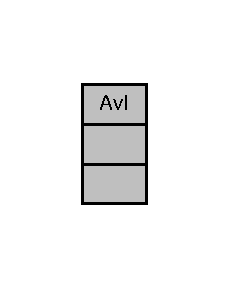
\includegraphics[width=110pt]{structAvl__coll__graph}
\end{center}
\end{figure}


\subsection{Detailed Description}
This is the structure for representing an A\-V\-L . 

This structure consists of\-:
\begin{DoxyItemize}
\item the label \-: an int
\item the son left \-: tree pointer
\item the son right \-: tree pointer
\item the height of the tree \-: an int 
\end{DoxyItemize}

The documentation for this struct was generated from the following file\-:\begin{DoxyCompactItemize}
\item 
\hyperlink{Core_8h}{Core.\-h}\end{DoxyCompactItemize}

\hypertarget{structBounds}{\section{Bounds Struct Reference}
\label{structBounds}\index{Bounds@{Bounds}}
}


Objet that represente bounds for an open street map.  




{\ttfamily \#include $<$Core.\-h$>$}



Collaboration diagram for Bounds\-:
\nopagebreak
\begin{figure}[H]
\begin{center}
\leavevmode
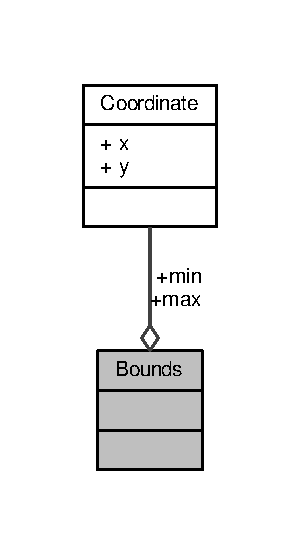
\includegraphics[width=144pt]{structBounds__coll__graph}
\end{center}
\end{figure}
\subsection*{Public Attributes}
\begin{DoxyCompactItemize}
\item 
\hypertarget{structBounds_a1c9164048f1f4c69c95fe140ade0b356}{\hyperlink{structCoordinate}{Coordinate} $\ast$ {\bfseries min}}\label{structBounds_a1c9164048f1f4c69c95fe140ade0b356}

\item 
\hypertarget{structBounds_a78e28f17202532fe18c6d05cc155c791}{\hyperlink{structCoordinate}{Coordinate} $\ast$ {\bfseries max}}\label{structBounds_a78e28f17202532fe18c6d05cc155c791}

\end{DoxyCompactItemize}


\subsection{Detailed Description}
Objet that represente bounds for an open street map. 

min is the coordinates of the minimum's point that it can have max is the coordinates of the maximum's point that it can have 

The documentation for this struct was generated from the following file\-:\begin{DoxyCompactItemize}
\item 
\hyperlink{Core_8h}{Core.\-h}\end{DoxyCompactItemize}

\hypertarget{structColor}{\section{Color Struct Reference}
\label{structColor}\index{Color@{Color}}
}


Objet that represente color in rgb.  




{\ttfamily \#include $<$Core.\-h$>$}

\subsection*{Public Attributes}
\begin{DoxyCompactItemize}
\item 
\hypertarget{structColor_a3cd71f006939f83ecd756f0ed28db40e}{int {\bfseries red}}\label{structColor_a3cd71f006939f83ecd756f0ed28db40e}

\item 
\hypertarget{structColor_afc8d0d81900a12497d1ce001e52b7020}{int {\bfseries green}}\label{structColor_afc8d0d81900a12497d1ce001e52b7020}

\item 
\hypertarget{structColor_a51f2c5eb0ffc788331255fa1c7812880}{int {\bfseries blue}}\label{structColor_a51f2c5eb0ffc788331255fa1c7812880}

\end{DoxyCompactItemize}


\subsection{Detailed Description}
Objet that represente color in rgb. 

red is the proportion of red in the color green is the proportion of green in the color bleu is the proportion of bleu in the color 

The documentation for this struct was generated from the following file\-:\begin{DoxyCompactItemize}
\item 
\hyperlink{Core_8h}{Core.\-h}\end{DoxyCompactItemize}

\hypertarget{structCoordinate}{\section{Coordinate Struct Reference}
\label{structCoordinate}\index{Coordinate@{Coordinate}}
}


Objet that represente the coordinate of a point.  




{\ttfamily \#include $<$Core.\-h$>$}

\subsection*{Public Attributes}
\begin{DoxyCompactItemize}
\item 
\hypertarget{structCoordinate_a514c8968b1d03f65e76c9cc9566ee4cc}{float {\bfseries x}}\label{structCoordinate_a514c8968b1d03f65e76c9cc9566ee4cc}

\item 
\hypertarget{structCoordinate_a1a7d11305e68c5bfba2b9d4569d4b6ef}{float {\bfseries y}}\label{structCoordinate_a1a7d11305e68c5bfba2b9d4569d4b6ef}

\end{DoxyCompactItemize}


\subsection{Detailed Description}
Objet that represente the coordinate of a point. 

x is the abscissa's coordinate y is the ordely's coordinate 

The documentation for this struct was generated from the following file\-:\begin{DoxyCompactItemize}
\item 
\hyperlink{Core_8h}{Core.\-h}\end{DoxyCompactItemize}

\hypertarget{structList}{\section{List Struct Reference}
\label{structList}\index{List@{List}}
}


Objet that represente a \hyperlink{structList}{List} of \hyperlink{structWay}{Way}.  




{\ttfamily \#include $<$Core.\-h$>$}



Collaboration diagram for List\-:
\nopagebreak
\begin{figure}[H]
\begin{center}
\leavevmode
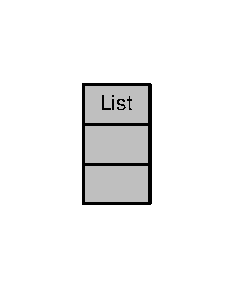
\includegraphics[width=112pt]{structList__coll__graph}
\end{center}
\end{figure}


\subsection{Detailed Description}
Objet that represente a \hyperlink{structList}{List} of \hyperlink{structWay}{Way}. 

Objet that represente a \hyperlink{structList}{List} of \hyperlink{structRelation}{Relation}.

first\-Ref is the first \hyperlink{structWay}{Way} of the \hyperlink{structList}{List} last\-Ref is the last \hyperlink{structWay}{Way} of the \hyperlink{structList}{List}

first\-Ref is the first \hyperlink{structRelation}{Relation} of the \hyperlink{structList}{List} last\-Ref is the last \hyperlink{structRelation}{Relation} of the \hyperlink{structList}{List} 

The documentation for this struct was generated from the following file\-:\begin{DoxyCompactItemize}
\item 
\hyperlink{Core_8h}{Core.\-h}\end{DoxyCompactItemize}

\hypertarget{structListNode}{\section{List\-Node Struct Reference}
\label{structListNode}\index{List\-Node@{List\-Node}}
}


Objet that represente a \hyperlink{structList}{List} of \hyperlink{structNode}{Node}.  




{\ttfamily \#include $<$Core.\-h$>$}



Collaboration diagram for List\-Node\-:
\nopagebreak
\begin{figure}[H]
\begin{center}
\leavevmode
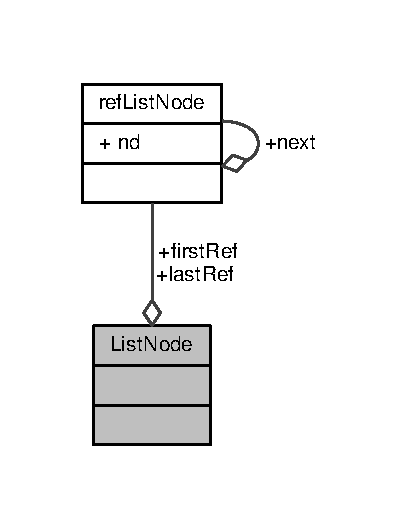
\includegraphics[width=192pt]{structListNode__coll__graph}
\end{center}
\end{figure}
\subsection*{Public Attributes}
\begin{DoxyCompactItemize}
\item 
\hypertarget{structListNode_a4264652974ed589c9ed582f3a4824601}{\hyperlink{structrefListNode}{ref\-List\-Node} $\ast$ {\bfseries first\-Ref}}\label{structListNode_a4264652974ed589c9ed582f3a4824601}

\item 
\hypertarget{structListNode_a014039589e69b8826362231855e4d96d}{\hyperlink{structrefListNode}{ref\-List\-Node} $\ast$ {\bfseries last\-Ref}}\label{structListNode_a014039589e69b8826362231855e4d96d}

\end{DoxyCompactItemize}


\subsection{Detailed Description}
Objet that represente a \hyperlink{structList}{List} of \hyperlink{structNode}{Node}. 

first\-Ref is the first \hyperlink{structNode}{Node} of the \hyperlink{structList}{List} last\-Ref is the last \hyperlink{structNode}{Node} of the \hyperlink{structList}{List} 

The documentation for this struct was generated from the following file\-:\begin{DoxyCompactItemize}
\item 
\hyperlink{Core_8h}{Core.\-h}\end{DoxyCompactItemize}

\hypertarget{structListRelation}{\section{List\-Relation Struct Reference}
\label{structListRelation}\index{List\-Relation@{List\-Relation}}
}


Collaboration diagram for List\-Relation\-:
\nopagebreak
\begin{figure}[H]
\begin{center}
\leavevmode
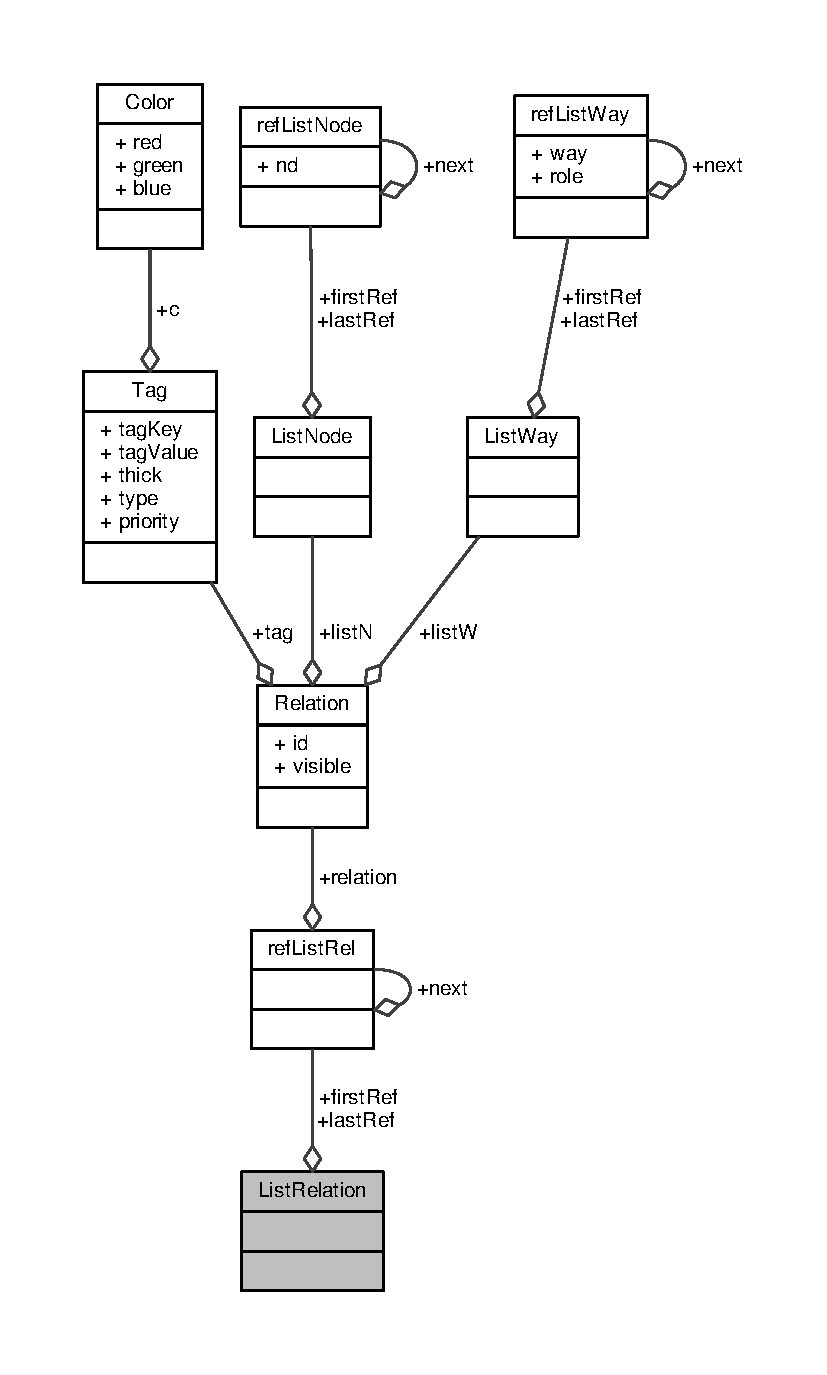
\includegraphics[height=550pt]{structListRelation__coll__graph}
\end{center}
\end{figure}
\subsection*{Public Attributes}
\begin{DoxyCompactItemize}
\item 
\hypertarget{structListRelation_a9de99495f108f7572e94513904e89478}{\hyperlink{structrefListRel}{ref\-List\-Rel} $\ast$ {\bfseries first\-Ref}}\label{structListRelation_a9de99495f108f7572e94513904e89478}

\item 
\hypertarget{structListRelation_a817271b56fb219729619f60c982dc4ec}{\hyperlink{structrefListRel}{ref\-List\-Rel} $\ast$ {\bfseries last\-Ref}}\label{structListRelation_a817271b56fb219729619f60c982dc4ec}

\end{DoxyCompactItemize}


The documentation for this struct was generated from the following file\-:\begin{DoxyCompactItemize}
\item 
\hyperlink{Core_8h}{Core.\-h}\end{DoxyCompactItemize}

\hypertarget{structListWay}{\section{List\-Way Struct Reference}
\label{structListWay}\index{List\-Way@{List\-Way}}
}
\subsection*{Public Attributes}
\begin{DoxyCompactItemize}
\item 
\hypertarget{structListWay_a5864089678f85dee9cac7dcbb651c760}{\hyperlink{structrefListWay}{ref\-List\-Way} $\ast$ {\bfseries first\-Ref}}\label{structListWay_a5864089678f85dee9cac7dcbb651c760}

\item 
\hypertarget{structListWay_af314caeee839f16f5b489a0ec34cba44}{\hyperlink{structrefListWay}{ref\-List\-Way} $\ast$ {\bfseries last\-Ref}}\label{structListWay_af314caeee839f16f5b489a0ec34cba44}

\end{DoxyCompactItemize}


The documentation for this struct was generated from the following file\-:\begin{DoxyCompactItemize}
\item 
\hyperlink{Core_8h}{Core.\-h}\end{DoxyCompactItemize}

\hypertarget{structMap}{\section{Map Struct Reference}
\label{structMap}\index{Map@{Map}}
}


This is the structure for representing a \hyperlink{structMap}{Map} from Openstreet\-Map . \hyperlink{structBounds}{Bounds} of a \hyperlink{structMap}{Map} \hyperlink{structAvl}{Avl} of \hyperlink{structNode}{Node} \hyperlink{structAvl}{Avl} of \hyperlink{structWay}{Way} \hyperlink{structList}{List} \hyperlink{structWay}{Way} \hyperlink{structList}{List} of relation Table of \hyperlink{structTag}{Tag} that represente the principal tag and their particularities.  




{\ttfamily \#include $<$Core.\-h$>$}

\subsection*{Public Attributes}
\begin{DoxyCompactItemize}
\item 
\hypertarget{structMap_a8f2c15a0ea06301fc805cd205342e2e0}{\hyperlink{structBounds}{Bounds} $\ast$ {\bfseries bounds}}\label{structMap_a8f2c15a0ea06301fc805cd205342e2e0}

\item 
\hypertarget{structMap_a58fbe72e5912e6d2cd418769486808a5}{\hyperlink{structAvl}{Avl} $\ast$ {\bfseries avl}}\label{structMap_a58fbe72e5912e6d2cd418769486808a5}

\item 
\hypertarget{structMap_ae62dcd5359ef0ec017dfc8cf19c19346}{\hyperlink{structAvl}{Avl} $\ast$ {\bfseries avl\-Way}}\label{structMap_ae62dcd5359ef0ec017dfc8cf19c19346}

\item 
\hypertarget{structMap_a3af2f22162a2e43f338ff21f2658443e}{\hyperlink{structListWay}{List\-Way} $\ast$ {\bfseries way\-Other}}\label{structMap_a3af2f22162a2e43f338ff21f2658443e}

\item 
\hypertarget{structMap_a960f6fdcdf754b044fb5f88030d7ac26}{\hyperlink{structListWay}{List\-Way} $\ast$ {\bfseries way\-Water}}\label{structMap_a960f6fdcdf754b044fb5f88030d7ac26}

\item 
\hypertarget{structMap_a79d06fbed6bdfa0f5195fc00c4ff4aa9}{\hyperlink{structListWay}{List\-Way} $\ast$ {\bfseries way\-Green}}\label{structMap_a79d06fbed6bdfa0f5195fc00c4ff4aa9}

\item 
\hypertarget{structMap_accbeabbfbcf2eb0a793a775f2903af1b}{\hyperlink{structListWay}{List\-Way} $\ast$ {\bfseries way\-Highway}}\label{structMap_accbeabbfbcf2eb0a793a775f2903af1b}

\item 
\hypertarget{structMap_a041101a912792f96b93693cecbbd2dca}{\hyperlink{structListWay}{List\-Way} $\ast$ {\bfseries way\-Building}}\label{structMap_a041101a912792f96b93693cecbbd2dca}

\item 
\hypertarget{structMap_ae6bc84ef3523d7660f6e1920058bf7af}{\hyperlink{structListWay}{List\-Way} $\ast$ {\bfseries way\-Cadastre}}\label{structMap_ae6bc84ef3523d7660f6e1920058bf7af}

\item 
\hypertarget{structMap_a8d2ebc0ae7299d72d43126d5a4b79b85}{\hyperlink{structListRelation}{List\-Relation} $\ast$ {\bfseries list\-Relation}}\label{structMap_a8d2ebc0ae7299d72d43126d5a4b79b85}

\item 
\hypertarget{structMap_aa53f6ae8f105ee942028395514f54e18}{\hyperlink{structTag}{Tag} $\ast$$\ast$ {\bfseries reference\-Tag}}\label{structMap_aa53f6ae8f105ee942028395514f54e18}

\end{DoxyCompactItemize}


\subsection{Detailed Description}
This is the structure for representing a \hyperlink{structMap}{Map} from Openstreet\-Map . \hyperlink{structBounds}{Bounds} of a \hyperlink{structMap}{Map} \hyperlink{structAvl}{Avl} of \hyperlink{structNode}{Node} \hyperlink{structAvl}{Avl} of \hyperlink{structWay}{Way} \hyperlink{structList}{List} \hyperlink{structWay}{Way} \hyperlink{structList}{List} of relation Table of \hyperlink{structTag}{Tag} that represente the principal tag and their particularities. 

The documentation for this struct was generated from the following file\-:\begin{DoxyCompactItemize}
\item 
\hyperlink{Core_8h}{Core.\-h}\end{DoxyCompactItemize}

\hypertarget{structNode}{\section{Node Struct Reference}
\label{structNode}\index{Node@{Node}}
}


Objet that represente a point in openstreetmap.  




{\ttfamily \#include $<$Core.\-h$>$}



Collaboration diagram for Node\-:
\nopagebreak
\begin{figure}[H]
\begin{center}
\leavevmode
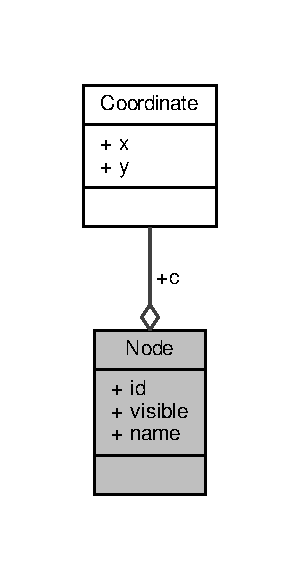
\includegraphics[width=144pt]{structNode__coll__graph}
\end{center}
\end{figure}
\subsection*{Public Attributes}
\begin{DoxyCompactItemize}
\item 
\hypertarget{structNode_aa8fa6b7f98e29166dbccce4a7f09929c}{unsigned long {\bfseries id}}\label{structNode_aa8fa6b7f98e29166dbccce4a7f09929c}

\item 
\hypertarget{structNode_a26b699d982158ab6f00cff23b1e13d4b}{\hyperlink{structCoordinate}{Coordinate} $\ast$ {\bfseries c}}\label{structNode_a26b699d982158ab6f00cff23b1e13d4b}

\item 
\hypertarget{structNode_a028bca5291cb35567d02b8077a81efdb}{char $\ast$ {\bfseries visible}}\label{structNode_a028bca5291cb35567d02b8077a81efdb}

\item 
\hypertarget{structNode_a059a0ea6f86dce9fd919c08a707b360b}{char $\ast$ {\bfseries name}}\label{structNode_a059a0ea6f86dce9fd919c08a707b360b}

\end{DoxyCompactItemize}


\subsection{Detailed Description}
Objet that represente a point in openstreetmap. 

id represente the name of this object c represente where is this point on the map visible represente if this point is visible or not name is the char $\ast$ with represente the name of node 

The documentation for this struct was generated from the following file\-:\begin{DoxyCompactItemize}
\item 
\hyperlink{Core_8h}{Core.\-h}\end{DoxyCompactItemize}

\hypertarget{structrefList}{\section{ref\-List Struct Reference}
\label{structrefList}\index{ref\-List@{ref\-List}}
}


Objet that represente a \hyperlink{structNode}{Node} and the next \hyperlink{structNode}{Node}.  




{\ttfamily \#include $<$Core.\-h$>$}



\subsection{Detailed Description}
Objet that represente a \hyperlink{structNode}{Node} and the next \hyperlink{structNode}{Node}. 

nd is the principal id \hyperlink{structNode}{Node} next is the next \hyperlink{structNode}{Node} 

The documentation for this struct was generated from the following file\-:\begin{DoxyCompactItemize}
\item 
\hyperlink{Core_8h}{Core.\-h}\end{DoxyCompactItemize}

\hypertarget{structrefListNode}{\section{ref\-List\-Node Struct Reference}
\label{structrefListNode}\index{ref\-List\-Node@{ref\-List\-Node}}
}


Collaboration diagram for ref\-List\-Node\-:
\nopagebreak
\begin{figure}[H]
\begin{center}
\leavevmode
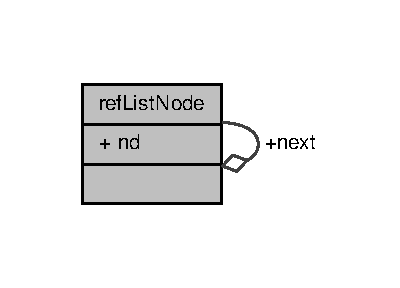
\includegraphics[width=192pt]{structrefListNode__coll__graph}
\end{center}
\end{figure}
\subsection*{Public Attributes}
\begin{DoxyCompactItemize}
\item 
\hypertarget{structrefListNode_aad950dd70f5d0b14f39b1f67dfc01580}{unsigned long {\bfseries nd}}\label{structrefListNode_aad950dd70f5d0b14f39b1f67dfc01580}

\item 
\hypertarget{structrefListNode_abc7e153a5f4c6f5652cecd19da99cbce}{struct \hyperlink{structrefListNode}{ref\-List\-Node} $\ast$ {\bfseries next}}\label{structrefListNode_abc7e153a5f4c6f5652cecd19da99cbce}

\end{DoxyCompactItemize}


The documentation for this struct was generated from the following file\-:\begin{DoxyCompactItemize}
\item 
\hyperlink{Core_8h}{Core.\-h}\end{DoxyCompactItemize}

\hypertarget{structrefListRel}{\section{ref\-List\-Rel Struct Reference}
\label{structrefListRel}\index{ref\-List\-Rel@{ref\-List\-Rel}}
}


Objet that represente a long and the next long (id)  




{\ttfamily \#include $<$Core.\-h$>$}



Collaboration diagram for ref\-List\-Rel\-:
\nopagebreak
\begin{figure}[H]
\begin{center}
\leavevmode
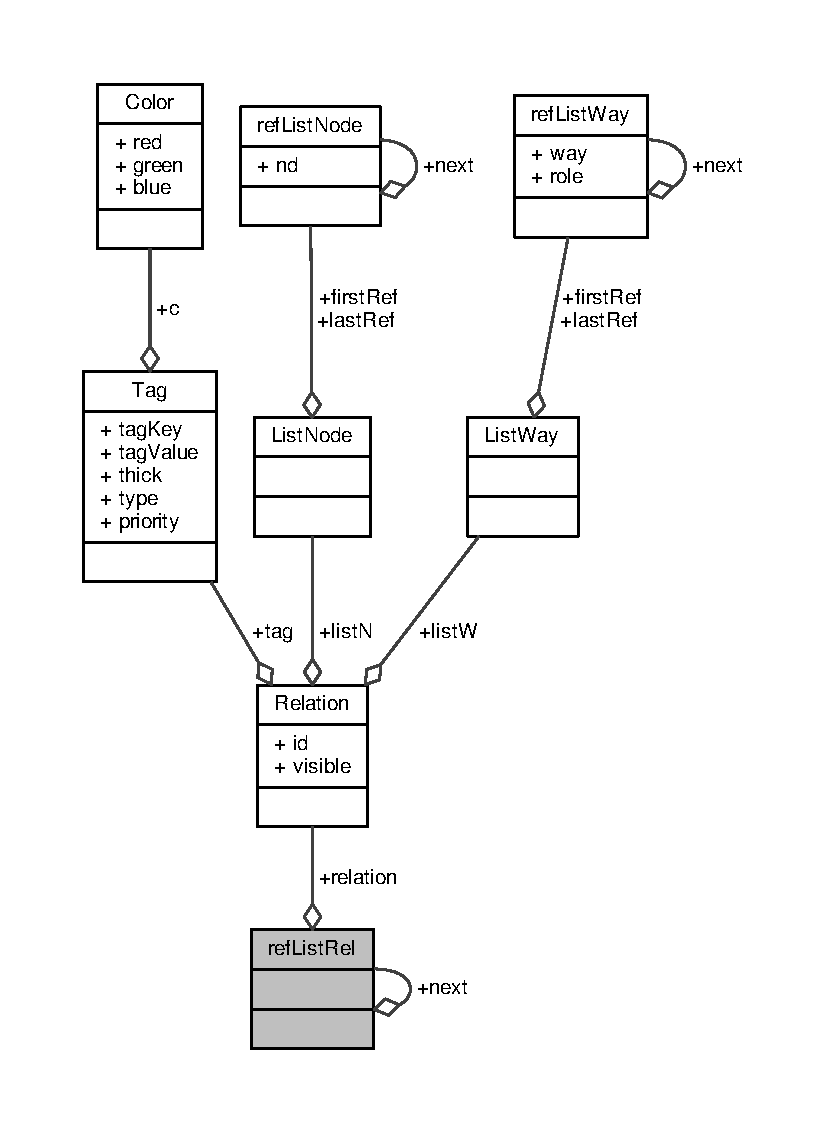
\includegraphics[width=350pt]{structrefListRel__coll__graph}
\end{center}
\end{figure}
\subsection*{Public Attributes}
\begin{DoxyCompactItemize}
\item 
\hypertarget{structrefListRel_a9598a4aceb866d060f6b4425e2d926d3}{\hyperlink{structRelation}{Relation} $\ast$ {\bfseries relation}}\label{structrefListRel_a9598a4aceb866d060f6b4425e2d926d3}

\item 
\hypertarget{structrefListRel_aa108a14d477cc8fc9706a7b535879cf8}{struct \hyperlink{structrefListRel}{ref\-List\-Rel} $\ast$ {\bfseries next}}\label{structrefListRel_aa108a14d477cc8fc9706a7b535879cf8}

\end{DoxyCompactItemize}


\subsection{Detailed Description}
Objet that represente a long and the next long (id) 

\hyperlink{structRelation}{Relation} is the principal relation next is the next relation 

The documentation for this struct was generated from the following file\-:\begin{DoxyCompactItemize}
\item 
\hyperlink{Core_8h}{Core.\-h}\end{DoxyCompactItemize}

\hypertarget{structrefListWay}{\section{ref\-List\-Way Struct Reference}
\label{structrefListWay}\index{ref\-List\-Way@{ref\-List\-Way}}
}


Objet that represente a long and the next long (id)  




{\ttfamily \#include $<$Core.\-h$>$}

\subsection*{Public Attributes}
\begin{DoxyCompactItemize}
\item 
\hypertarget{structrefListWay_ab4efd61c3ba5bfd6a68aec29ae9ffef0}{unsigned long {\bfseries way}}\label{structrefListWay_ab4efd61c3ba5bfd6a68aec29ae9ffef0}

\item 
\hypertarget{structrefListWay_a1a091291a89a5f54ba76b4e4bdcbe7b1}{char $\ast$ {\bfseries role}}\label{structrefListWay_a1a091291a89a5f54ba76b4e4bdcbe7b1}

\item 
\hypertarget{structrefListWay_aa0b05de016593f1b96812a8ba93fe9ff}{struct \hyperlink{structrefListWay}{ref\-List\-Way} $\ast$ {\bfseries next}}\label{structrefListWay_aa0b05de016593f1b96812a8ba93fe9ff}

\end{DoxyCompactItemize}


\subsection{Detailed Description}
Objet that represente a long and the next long (id) 

way is the principal way role is the role of the way next is the next way 

The documentation for this struct was generated from the following file\-:\begin{DoxyCompactItemize}
\item 
\hyperlink{Core_8h}{Core.\-h}\end{DoxyCompactItemize}

\hypertarget{structRelation}{\section{Relation Struct Reference}
\label{structRelation}\index{Relation@{Relation}}
}


Objet that represente a construction like a building or a garden in openstreetmap.  




{\ttfamily \#include $<$Core.\-h$>$}



Collaboration diagram for Relation\-:
\nopagebreak
\begin{figure}[H]
\begin{center}
\leavevmode
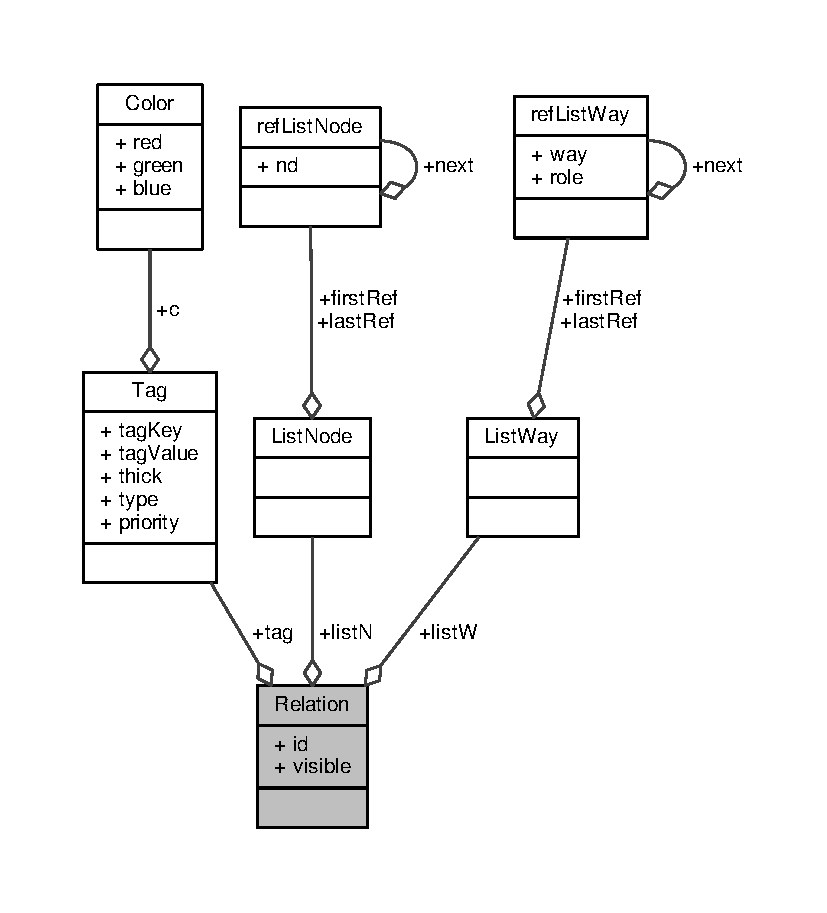
\includegraphics[width=350pt]{structRelation__coll__graph}
\end{center}
\end{figure}
\subsection*{Public Attributes}
\begin{DoxyCompactItemize}
\item 
\hypertarget{structRelation_a3f70b867d03c79bfa4dc98516ef1c25f}{unsigned long {\bfseries id}}\label{structRelation_a3f70b867d03c79bfa4dc98516ef1c25f}

\item 
\hypertarget{structRelation_a9a569cd7a800102a952b61bafe3f5fa7}{\hyperlink{structListWay}{List\-Way} $\ast$ {\bfseries list\-W}}\label{structRelation_a9a569cd7a800102a952b61bafe3f5fa7}

\item 
\hypertarget{structRelation_a55c4f77df17c7ab272ee93db476e8c8f}{\hyperlink{structListNode}{List\-Node} $\ast$ {\bfseries list\-N}}\label{structRelation_a55c4f77df17c7ab272ee93db476e8c8f}

\item 
\hypertarget{structRelation_af672e16f4fb0a93645b784e171f991d4}{\hyperlink{structTag}{Tag} $\ast$ {\bfseries tag}}\label{structRelation_af672e16f4fb0a93645b784e171f991d4}

\item 
\hypertarget{structRelation_a54cd0470aa40ddc3872899edcdd70eb1}{char $\ast$ {\bfseries visible}}\label{structRelation_a54cd0470aa40ddc3872899edcdd70eb1}

\end{DoxyCompactItemize}


\subsection{Detailed Description}
Objet that represente a construction like a building or a garden in openstreetmap. 

id represente the name of this object list\-W is the list of the differents way that it compose this object list\-N is the list of the differents node that it compose this object visible represente if this point is visible or not tag is the type of this object 

The documentation for this struct was generated from the following file\-:\begin{DoxyCompactItemize}
\item 
\hyperlink{Core_8h}{Core.\-h}\end{DoxyCompactItemize}

\hypertarget{structsAvl}{\section{s\-Avl Struct Reference}
\label{structsAvl}\index{s\-Avl@{s\-Avl}}
}


Collaboration diagram for s\-Avl\-:
\nopagebreak
\begin{figure}[H]
\begin{center}
\leavevmode
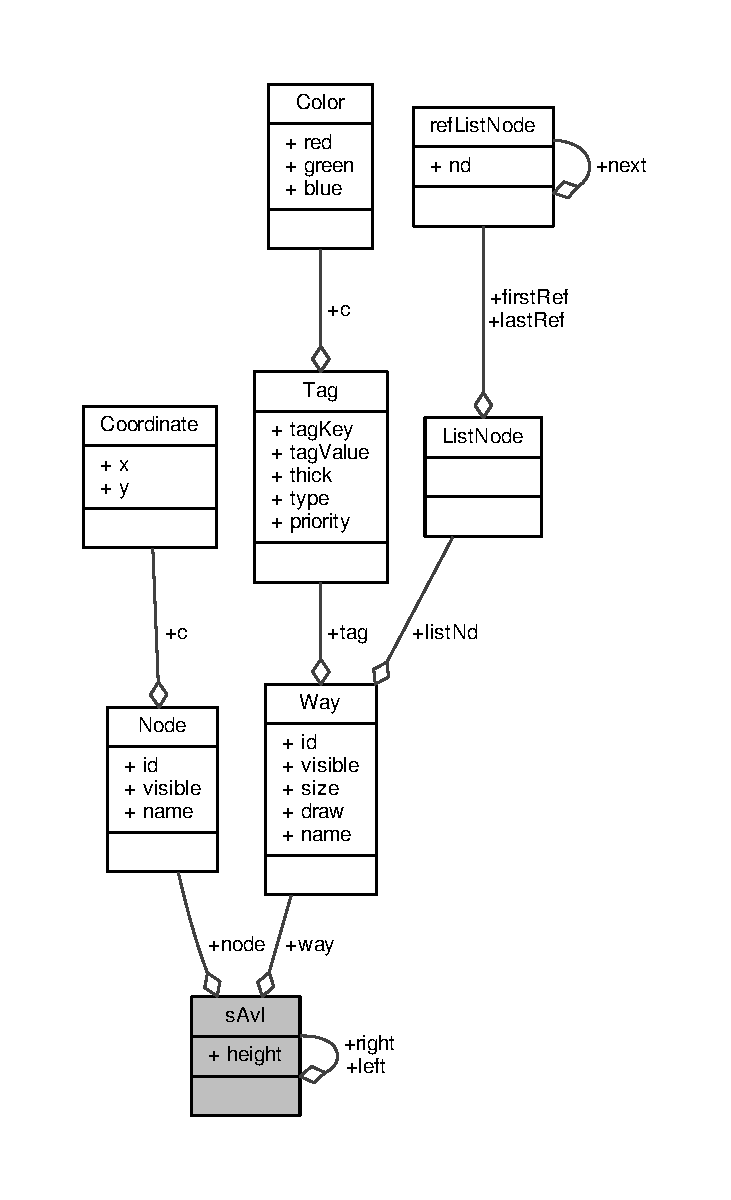
\includegraphics[height=550pt]{structsAvl__coll__graph}
\end{center}
\end{figure}
\subsection*{Public Attributes}
\begin{DoxyCompactItemize}
\item 
\hypertarget{structsAvl_a86e4262b6dcb6d69a23274064a90c2c7}{\hyperlink{structNode}{Node} $\ast$ {\bfseries node}}\label{structsAvl_a86e4262b6dcb6d69a23274064a90c2c7}

\item 
\hypertarget{structsAvl_a1f65b88ea657e036d81dd9587b1f7566}{\hyperlink{structWay}{Way} $\ast$ {\bfseries way}}\label{structsAvl_a1f65b88ea657e036d81dd9587b1f7566}

\item 
\hypertarget{structsAvl_a1678d05e6984326e3f25002f9b5d4ac9}{int {\bfseries height}}\label{structsAvl_a1678d05e6984326e3f25002f9b5d4ac9}

\item 
\hypertarget{structsAvl_a97ab2166bf624b8cc03c6a02ba46ea9d}{struct \hyperlink{structsAvl}{s\-Avl} $\ast$ {\bfseries left}}\label{structsAvl_a97ab2166bf624b8cc03c6a02ba46ea9d}

\item 
\hypertarget{structsAvl_a251c789fc0532eae2b7a6fadd64d39a4}{struct \hyperlink{structsAvl}{s\-Avl} $\ast$ {\bfseries right}}\label{structsAvl_a251c789fc0532eae2b7a6fadd64d39a4}

\end{DoxyCompactItemize}


The documentation for this struct was generated from the following file\-:\begin{DoxyCompactItemize}
\item 
\hyperlink{Core_8h}{Core.\-h}\end{DoxyCompactItemize}

\hypertarget{structTag}{\section{Tag Struct Reference}
\label{structTag}\index{Tag@{Tag}}
}


Objet that represente tags for an open street map.  




{\ttfamily \#include $<$Core.\-h$>$}



Collaboration diagram for Tag\-:
\nopagebreak
\begin{figure}[H]
\begin{center}
\leavevmode
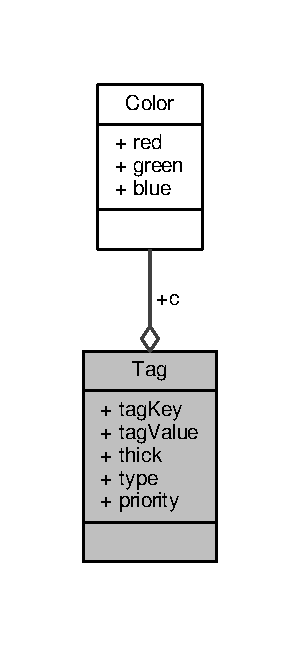
\includegraphics[width=144pt]{structTag__coll__graph}
\end{center}
\end{figure}
\subsection*{Public Attributes}
\begin{DoxyCompactItemize}
\item 
\hypertarget{structTag_a9e91de69887dba3f1a2e9d532acbce8b}{char $\ast$ {\bfseries tag\-Key}}\label{structTag_a9e91de69887dba3f1a2e9d532acbce8b}

\item 
\hypertarget{structTag_ace008f9a4f15d8128de404a0c920ab0d}{char $\ast$ {\bfseries tag\-Value}}\label{structTag_ace008f9a4f15d8128de404a0c920ab0d}

\item 
\hypertarget{structTag_a6805504ea08ce816b95c5441f7485348}{\hyperlink{structColor}{Color} $\ast$ {\bfseries c}}\label{structTag_a6805504ea08ce816b95c5441f7485348}

\item 
\hypertarget{structTag_a6456de00a94753379709078b718a8724}{int {\bfseries thick}}\label{structTag_a6456de00a94753379709078b718a8724}

\item 
\hypertarget{structTag_acd71a132bb412efeccfbc87b3cc25787}{int {\bfseries type}}\label{structTag_acd71a132bb412efeccfbc87b3cc25787}

\item 
\hypertarget{structTag_af4bf844100277f4167d6cbe2d83d879d}{int {\bfseries priority}}\label{structTag_af4bf844100277f4167d6cbe2d83d879d}

\end{DoxyCompactItemize}


\subsection{Detailed Description}
Objet that represente tags for an open street map. 

tag\-Key is the key of the tags tag\-Value is the value of the tags \hyperlink{structColor}{Color} is the color of this type of element thick represente the thickness of the way type represente the type of the tag to know in which list\-Way it have to be \-: 1=water, 2=green, 3=highway, 4= building, 0=other; priority represente the priority of have this tag, it permit to choose the better tag 

The documentation for this struct was generated from the following file\-:\begin{DoxyCompactItemize}
\item 
\hyperlink{Core_8h}{Core.\-h}\end{DoxyCompactItemize}

\hypertarget{structWay}{\section{Way Struct Reference}
\label{structWay}\index{Way@{Way}}
}


Objet that represente a construction like a building or a garden in openstreetmap.  




{\ttfamily \#include $<$Core.\-h$>$}

\subsection*{Public Attributes}
\begin{DoxyCompactItemize}
\item 
\hypertarget{structWay_a1cca095d0625e82d6bfb36dd1d46640f}{unsigned long {\bfseries id}}\label{structWay_a1cca095d0625e82d6bfb36dd1d46640f}

\item 
\hypertarget{structWay_acac0fa32ab84a83dd2797fb255a4fe1a}{\hyperlink{structListNode}{List\-Node} $\ast$ {\bfseries list\-Nd}}\label{structWay_acac0fa32ab84a83dd2797fb255a4fe1a}

\item 
\hypertarget{structWay_a1eb964f25274018f981f08292cb221bb}{char $\ast$ {\bfseries visible}}\label{structWay_a1eb964f25274018f981f08292cb221bb}

\item 
\hypertarget{structWay_a0941af436e8c52be813a29f02f0eb987}{\hyperlink{structTag}{Tag} $\ast$ {\bfseries tag}}\label{structWay_a0941af436e8c52be813a29f02f0eb987}

\item 
\hypertarget{structWay_a51e8d4755a7e591657d7e70f34984af0}{int {\bfseries size}}\label{structWay_a51e8d4755a7e591657d7e70f34984af0}

\item 
\hypertarget{structWay_a9bbbf5fb49a0c87e2672dad52d845839}{int {\bfseries draw}}\label{structWay_a9bbbf5fb49a0c87e2672dad52d845839}

\item 
\hypertarget{structWay_adedae7524ea19d540ad71fa905729697}{char $\ast$ {\bfseries name}}\label{structWay_adedae7524ea19d540ad71fa905729697}

\end{DoxyCompactItemize}


\subsection{Detailed Description}
Objet that represente a construction like a building or a garden in openstreetmap. 

id represente the name of this object list\-Nd is the list of the differents node that it compose this object visible represente if this point is visible or not tag is the type of this object size is the number of \hyperlink{structNode}{Node} draw egal 0 if the tag was never draw else 1 

The documentation for this struct was generated from the following file\-:\begin{DoxyCompactItemize}
\item 
\hyperlink{Core_8h}{Core.\-h}\end{DoxyCompactItemize}

\chapter{File Documentation}
\hypertarget{Avl_8h}{\section{Avl.\-h File Reference}
\label{Avl_8h}\index{Avl.\-h@{Avl.\-h}}
}


This file can create, insert and retrieve nodes in an \hyperlink{structAvl}{Avl} ( balanced binary tree search )  


{\ttfamily \#include $<$stdlib.\-h$>$}\\*
{\ttfamily \#include \char`\"{}init.\-h\char`\"{}}\\*
Include dependency graph for Avl.\-h\-:
\nopagebreak
\begin{figure}[H]
\begin{center}
\leavevmode
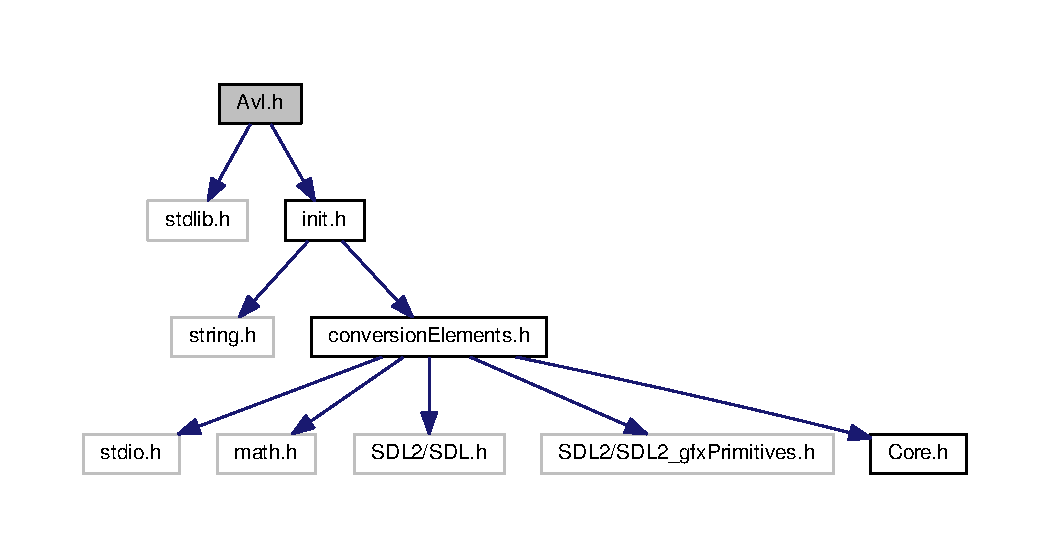
\includegraphics[width=350pt]{Avl_8h__incl}
\end{center}
\end{figure}
This graph shows which files directly or indirectly include this file\-:
\nopagebreak
\begin{figure}[H]
\begin{center}
\leavevmode
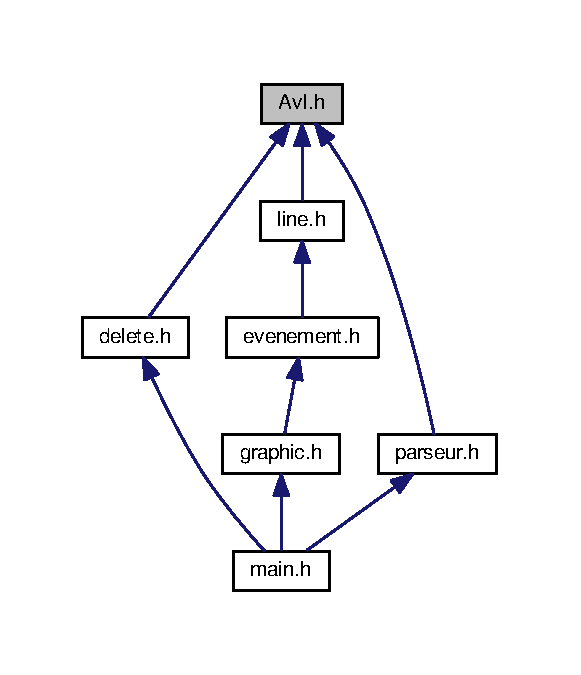
\includegraphics[width=279pt]{Avl_8h__dep__incl}
\end{center}
\end{figure}
\subsection*{Functions}
\begin{DoxyCompactItemize}
\item 
\hyperlink{structNode}{Node} $\ast$ \hyperlink{Avl_8h_a8e52d368bebcfc9c324c0ba0fa6d36c1}{search\-Node} (\hyperlink{structAvl}{Avl} $\ast$a, unsigned long key)
\item 
\hyperlink{structWay}{Way} $\ast$ \hyperlink{Avl_8h_a6ffec005bae68bcbbf4c5a35c26b2fc7}{search\-Way} (\hyperlink{structAvl}{Avl} $\ast$a, unsigned long key)
\item 
\hyperlink{structAvl}{Avl} $\ast$ \hyperlink{Avl_8h_ac32b350d2833f3ab0ba4ce82401a294c}{insert} (\hyperlink{structAvl}{Avl} $\ast$$\ast$a, \hyperlink{structNode}{Node} $\ast$n, \hyperlink{structWay}{Way} $\ast$w)
\item 
\hyperlink{structAvl}{Avl} $\ast$ \hyperlink{Avl_8h_aea98efe3919ecf1862aaf803d80daae1}{init} (\hyperlink{structAvl}{Avl} $\ast$$\ast$a, \hyperlink{structNode}{Node} $\ast$n, \hyperlink{structWay}{Way} $\ast$w)
\item 
void \hyperlink{Avl_8h_a8bc4ab41e0f9a381c6eba6de37b02a6f}{print\-Node} (\hyperlink{structAvl}{Avl} $\ast$$\ast$a, unsigned long nombre)
\item 
void \hyperlink{Avl_8h_af25e0f0f73416c86303d8d36f4416cf8}{print\-Way} (\hyperlink{structAvl}{Avl} $\ast$$\ast$a, unsigned long nombre)
\end{DoxyCompactItemize}


\subsection{Detailed Description}
This file can create, insert and retrieve nodes in an \hyperlink{structAvl}{Avl} ( balanced binary tree search ) \begin{DoxyAuthor}{Author}
Isabelle M\-A\-R\-I\-N\-O Pierrick J\-A\-C\-Q\-U\-E\-T\-T\-E Hafça T\-I\-R\-I\-C\-H\-I\-N\-E
\end{DoxyAuthor}
Basic operations of an A\-V\-L tree involve carrying out the same actions as would be carried out on an unbalanced binary search tree, but modifications are followed by zero or more operations called tree rotations, which help to restore the height balance of the subtrees.

The insertion, search are O(log n) 

\subsection{Function Documentation}
\hypertarget{Avl_8h_aea98efe3919ecf1862aaf803d80daae1}{\index{Avl.\-h@{Avl.\-h}!init@{init}}
\index{init@{init}!Avl.h@{Avl.\-h}}
\subsubsection[{init}]{\setlength{\rightskip}{0pt plus 5cm}{\bf Avl}$\ast$ init (
\begin{DoxyParamCaption}
\item[{{\bf Avl} $\ast$$\ast$}]{a, }
\item[{{\bf Node} $\ast$}]{n, }
\item[{{\bf Way} $\ast$}]{w}
\end{DoxyParamCaption}
)}}\label{Avl_8h_aea98efe3919ecf1862aaf803d80daae1}
Initializing the A\-V\-L with the root , the parameter content 
\begin{DoxyParams}{Parameters}
{\em a} & Self-\/balancing binary search tree \\
\hline
{\em n} & it is the reference node \\
\hline
{\em w} & it is the reference way \\
\hline
\end{DoxyParams}
\begin{DoxyReturn}{Returns}
A tree under the pointer with the change 
\end{DoxyReturn}


Here is the caller graph for this function\-:
\nopagebreak
\begin{figure}[H]
\begin{center}
\leavevmode
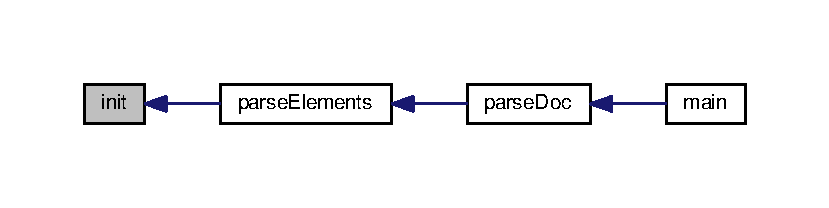
\includegraphics[width=350pt]{Avl_8h_aea98efe3919ecf1862aaf803d80daae1_icgraph}
\end{center}
\end{figure}


\hypertarget{Avl_8h_ac32b350d2833f3ab0ba4ce82401a294c}{\index{Avl.\-h@{Avl.\-h}!insert@{insert}}
\index{insert@{insert}!Avl.h@{Avl.\-h}}
\subsubsection[{insert}]{\setlength{\rightskip}{0pt plus 5cm}{\bf Avl}$\ast$ insert (
\begin{DoxyParamCaption}
\item[{{\bf Avl} $\ast$$\ast$}]{a, }
\item[{{\bf Node} $\ast$}]{n, }
\item[{{\bf Way} $\ast$}]{w}
\end{DoxyParamCaption}
)}}\label{Avl_8h_ac32b350d2833f3ab0ba4ce82401a294c}
function to insert the key in the A\-V\-L in the right place according to its value , and the transition if necessary, rebalanced the tree 
\begin{DoxyParams}{Parameters}
{\em a} & Self-\/balancing binary search tree \\
\hline
{\em n} & it is the reference node \\
\hline
{\em w} & it is the reference way \\
\hline
\end{DoxyParams}
\begin{DoxyReturn}{Returns}
A tree under the pointer with the change 
\end{DoxyReturn}


Here is the caller graph for this function\-:
\nopagebreak
\begin{figure}[H]
\begin{center}
\leavevmode
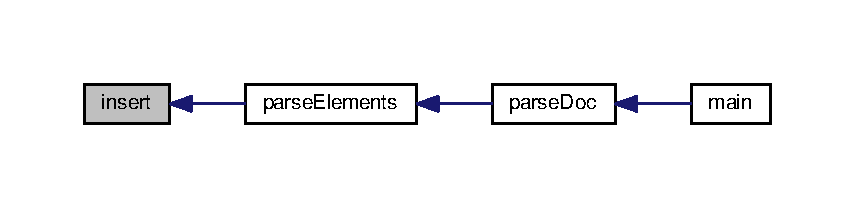
\includegraphics[width=350pt]{Avl_8h_ac32b350d2833f3ab0ba4ce82401a294c_icgraph}
\end{center}
\end{figure}


\hypertarget{Avl_8h_a8bc4ab41e0f9a381c6eba6de37b02a6f}{\index{Avl.\-h@{Avl.\-h}!print\-Node@{print\-Node}}
\index{print\-Node@{print\-Node}!Avl.h@{Avl.\-h}}
\subsubsection[{print\-Node}]{\setlength{\rightskip}{0pt plus 5cm}void print\-Node (
\begin{DoxyParamCaption}
\item[{{\bf Avl} $\ast$$\ast$}]{a, }
\item[{unsigned long}]{nombre}
\end{DoxyParamCaption}
)}}\label{Avl_8h_a8bc4ab41e0f9a381c6eba6de37b02a6f}
function allowing display of the A\-V\-L 
\begin{DoxyParams}{Parameters}
{\em a} & Self-\/balancing binary search tree \\
\hline
{\em nombre} & dentifier of the tree level view \\
\hline
\end{DoxyParams}
\hypertarget{Avl_8h_af25e0f0f73416c86303d8d36f4416cf8}{\index{Avl.\-h@{Avl.\-h}!print\-Way@{print\-Way}}
\index{print\-Way@{print\-Way}!Avl.h@{Avl.\-h}}
\subsubsection[{print\-Way}]{\setlength{\rightskip}{0pt plus 5cm}void print\-Way (
\begin{DoxyParamCaption}
\item[{{\bf Avl} $\ast$$\ast$}]{a, }
\item[{unsigned long}]{nombre}
\end{DoxyParamCaption}
)}}\label{Avl_8h_af25e0f0f73416c86303d8d36f4416cf8}
function allowing display of the A\-V\-L 
\begin{DoxyParams}{Parameters}
{\em a} & Self-\/balancing binary search tree \\
\hline
{\em nombre} & dentifier of the tree level view \\
\hline
\end{DoxyParams}
\hypertarget{Avl_8h_a8e52d368bebcfc9c324c0ba0fa6d36c1}{\index{Avl.\-h@{Avl.\-h}!search\-Node@{search\-Node}}
\index{search\-Node@{search\-Node}!Avl.h@{Avl.\-h}}
\subsubsection[{search\-Node}]{\setlength{\rightskip}{0pt plus 5cm}{\bf Node}$\ast$ search\-Node (
\begin{DoxyParamCaption}
\item[{{\bf Avl} $\ast$}]{a, }
\item[{unsigned long}]{key}
\end{DoxyParamCaption}
)}}\label{Avl_8h_a8e52d368bebcfc9c324c0ba0fa6d36c1}
search function in an A\-V\-L according to a key, this key is the reference node 
\begin{DoxyParams}{Parameters}
{\em a} & Self-\/balancing binary search tree \\
\hline
{\em key} & it is the reference node \\
\hline
\end{DoxyParams}
\begin{DoxyReturn}{Returns}
return the node if it exists, otherwise null 
\end{DoxyReturn}
\hypertarget{Avl_8h_a6ffec005bae68bcbbf4c5a35c26b2fc7}{\index{Avl.\-h@{Avl.\-h}!search\-Way@{search\-Way}}
\index{search\-Way@{search\-Way}!Avl.h@{Avl.\-h}}
\subsubsection[{search\-Way}]{\setlength{\rightskip}{0pt plus 5cm}{\bf Way}$\ast$ search\-Way (
\begin{DoxyParamCaption}
\item[{{\bf Avl} $\ast$}]{a, }
\item[{unsigned long}]{key}
\end{DoxyParamCaption}
)}}\label{Avl_8h_a6ffec005bae68bcbbf4c5a35c26b2fc7}
search function in an A\-V\-L according to a key, this key is the reference way 
\begin{DoxyParams}{Parameters}
{\em a} & Self-\/balancing binary search tree \\
\hline
{\em key} & it is the reference node \\
\hline
\end{DoxyParams}
\begin{DoxyReturn}{Returns}
return the way if it exists, otherwise null 
\end{DoxyReturn}

\hypertarget{conversionElements_8h}{\section{conversion\-Elements.\-h File Reference}
\label{conversionElements_8h}\index{conversion\-Elements.\-h@{conversion\-Elements.\-h}}
}


Declare fonctions to convert elements.  


{\ttfamily \#include $<$stdlib.\-h$>$}\\*
{\ttfamily \#include $<$math.\-h$>$}\\*
{\ttfamily \#include $<$S\-D\-L2/\-S\-D\-L.\-h$>$}\\*
{\ttfamily \#include $<$S\-D\-L2/\-S\-D\-L2\-\_\-gfx\-Primitives.\-h$>$}\\*
{\ttfamily \#include \char`\"{}Core.\-h\char`\"{}}\\*
\subsection*{Macros}
\begin{DoxyCompactItemize}
\item 
\hypertarget{conversionElements_8h_a0b4d28030851e5c6a15aae83dcad585c}{\#define {\bfseries P\-A\-S\-C\-L\-A\-V\-I\-E\-R}~10}\label{conversionElements_8h_a0b4d28030851e5c6a15aae83dcad585c}

\item 
\hypertarget{conversionElements_8h_a1144aeb2fb68d520a15c401ab2c75e7b}{\#define {\bfseries W\-I\-N\-D\-O\-W\-S\-\_\-\-W\-I\-D\-T\-H\-M\-I\-N}~100}\label{conversionElements_8h_a1144aeb2fb68d520a15c401ab2c75e7b}

\item 
\hypertarget{conversionElements_8h_ab384bd131e1670d9cf30e71200e7615b}{\#define {\bfseries W\-I\-N\-D\-O\-W\-S\-\_\-\-W\-I\-D\-T\-H\-M\-A\-X}~900}\label{conversionElements_8h_ab384bd131e1670d9cf30e71200e7615b}

\item 
\hypertarget{conversionElements_8h_a74511922386b54de0a6b3db99841aa3b}{\#define {\bfseries W\-I\-N\-D\-O\-W\-S\-\_\-\-H\-E\-I\-G\-H\-T\-M\-I\-N}~100}\label{conversionElements_8h_a74511922386b54de0a6b3db99841aa3b}

\item 
\hypertarget{conversionElements_8h_a6f1a8cfb4190c5fff3f18b7f2bc7eaac}{\#define {\bfseries W\-I\-N\-D\-O\-W\-S\-\_\-\-H\-E\-I\-G\-H\-T\-M\-A\-X}~700}\label{conversionElements_8h_a6f1a8cfb4190c5fff3f18b7f2bc7eaac}

\end{DoxyCompactItemize}
\subsection*{Functions}
\begin{DoxyCompactItemize}
\item 
\hyperlink{structCoordinate}{Coordinate} $\ast$ \hyperlink{conversionElements_8h_ad66d504f94bd54c34335365e98edd4e7}{conversion\-Lat\-Lon} (float lat, float lon)
\begin{DoxyCompactList}\small\item\em calculate the \hyperlink{structCoordinate}{Coordinate} for a point in openstreetmap \end{DoxyCompactList}\item 
\hyperlink{structBounds}{Bounds} $\ast$ \hyperlink{conversionElements_8h_a53a0d679e571c6851a5c6d0c7d37e763}{convert\-Bounds} (\hyperlink{structBounds}{Bounds} $\ast$b)
\begin{DoxyCompactList}\small\item\em convert the bounds of the map to the min is (0,0) \end{DoxyCompactList}\item 
float \hyperlink{conversionElements_8h_a78254a65bf2ec07b4268479ec6104c55}{distance\-X\-Y} (float x1, float y1, float x2, float y2)
\begin{DoxyCompactList}\small\item\em calculate the distance beetween 2 points in a carthesien repere \end{DoxyCompactList}\item 
float \hyperlink{conversionElements_8h_ae51377d214fc1d1063596883f0ed80ea}{distance\-Y} (float y1, float y2)
\begin{DoxyCompactList}\small\item\em calculate the ordinate's distance beetween 2 points in a carthesien repere \end{DoxyCompactList}\item 
float \hyperlink{conversionElements_8h_a075c229cf74f9814e529c85a425f2734}{distance\-X} (float x1, float x2)
\begin{DoxyCompactList}\small\item\em calculate the abscisse's distance beetween 2 points in a carthesien repere \end{DoxyCompactList}\item 
\hypertarget{conversionElements_8h_a953a883457e9906cfba52d505afbbe2b}{float {\bfseries normalize} (float a, float b, float length)}\label{conversionElements_8h_a953a883457e9906cfba52d505afbbe2b}

\item 
float \hyperlink{conversionElements_8h_a830c114c07e594b1b50f27627c98f5da}{angle} (float ax, float ay, float bx, float by, float cx, float cy)
\item 
\hyperlink{structNode}{Node} $\ast$ \hyperlink{conversionElements_8h_a248ef05c0bf1752dbdd368a8d3084ad9}{distance\-To\-Bounds} (\hyperlink{structBounds}{Bounds} $\ast$b, \hyperlink{structNode}{Node} $\ast$n)
\begin{DoxyCompactList}\small\item\em calcule the distance between a \hyperlink{structNode}{Node} and the \hyperlink{structBounds}{Bounds}'s map \end{DoxyCompactList}\item 
float \hyperlink{conversionElements_8h_a90591e521d718a45a88ec4b8d67a988b}{distance\-Lat\-Lon} (float lat1, float lon1, float lat2, float lon2)
\begin{DoxyCompactList}\small\item\em calculate the distance beetween 2 points in a map \end{DoxyCompactList}\item 
\hypertarget{conversionElements_8h_a023b9909d36d14d6f1693e4c437a0c51}{Sint16 $\ast$ {\bfseries midle} (float b, float e, int signe, Sint16 tab\mbox{[}4\mbox{]})}\label{conversionElements_8h_a023b9909d36d14d6f1693e4c437a0c51}

\item 
\hypertarget{conversionElements_8h_a04078c5a468feac011be27760f7c9d84}{Sint16 $\ast$ {\bfseries swap} (Sint16 tab\mbox{[}4\mbox{]})}\label{conversionElements_8h_a04078c5a468feac011be27760f7c9d84}

\item 
\hypertarget{conversionElements_8h_ac3e66c5ea95a9da290e4d89457724abf}{Sint16 $\ast$ {\bfseries extremite} (float a, float d, float e, Sint16 tab\mbox{[}4\mbox{]}, int signe, int extremite)}\label{conversionElements_8h_ac3e66c5ea95a9da290e4d89457724abf}

\item 
float \hyperlink{conversionElements_8h_a26f3232214f74a1eff1d8927c4f4b296}{mise\-A\-Echelle\-X} (float x, float y, int size)
\item 
float \hyperlink{conversionElements_8h_a4cb5ae2d71cf1e9c01b8439b5697e9d5}{mise\-A\-Echelle\-Y} (float x, float y, int size)
\item 
float \hyperlink{conversionElements_8h_a2851552394abaf56e2cc232660580e53}{calculate\-Zoom} (int ref\-X, int ref\-Y, float decalage, int flag)
\item 
int \hyperlink{conversionElements_8h_aa5c04722427362120674bd42606fbf9b}{color\-Background} (int red, int blue, int green, int oppacity)
\item 
int \hyperlink{conversionElements_8h_a9b565a29e63df82d12fae0a2a3f84349}{color\-Background\-Default} ()
\end{DoxyCompactItemize}
\subsection*{Variables}
\begin{DoxyCompactItemize}
\item 
\hypertarget{conversionElements_8h_a4063f0cc3259f847616fd638138216df}{int {\bfseries windows\-\_\-\-Height}}\label{conversionElements_8h_a4063f0cc3259f847616fd638138216df}

\item 
\hypertarget{conversionElements_8h_a443b5fae5439020c773c1f0e39354dbc}{int {\bfseries windows\-\_\-\-Width}}\label{conversionElements_8h_a443b5fae5439020c773c1f0e39354dbc}

\item 
\hypertarget{conversionElements_8h_aaa8e409e04dcf575ef63fd5fb3db06f9}{S\-D\-L\-\_\-\-Window $\ast$ {\bfseries window}}\label{conversionElements_8h_aaa8e409e04dcf575ef63fd5fb3db06f9}

\item 
\hypertarget{conversionElements_8h_a966da7a60c4ea3ba301e26ccc5efe452}{S\-D\-L\-\_\-\-Renderer $\ast$ {\bfseries renderer}}\label{conversionElements_8h_a966da7a60c4ea3ba301e26ccc5efe452}

\item 
\hypertarget{conversionElements_8h_a2896431d6a80cd39b3d24b40237612ee}{int {\bfseries quit}}\label{conversionElements_8h_a2896431d6a80cd39b3d24b40237612ee}

\item 
\hypertarget{conversionElements_8h_a51c5a239ff83d14d16f49f8ebd9e0a24}{int {\bfseries deplac\-X}}\label{conversionElements_8h_a51c5a239ff83d14d16f49f8ebd9e0a24}

\item 
\hypertarget{conversionElements_8h_ad8cc417990fc387a0d9f869c31c30453}{int {\bfseries deplac\-Y}}\label{conversionElements_8h_ad8cc417990fc387a0d9f869c31c30453}

\item 
\hypertarget{conversionElements_8h_a15776f201dc8b554110222e67a51cbae}{float {\bfseries zoom}}\label{conversionElements_8h_a15776f201dc8b554110222e67a51cbae}

\item 
\hypertarget{conversionElements_8h_ad7479fac074a257102bfd447e67fdff6}{int {\bfseries pas\-Souris\-X}}\label{conversionElements_8h_ad7479fac074a257102bfd447e67fdff6}

\item 
\hypertarget{conversionElements_8h_a958d1dedb8459e6f32b9d17711340199}{int {\bfseries pas\-Souris\-Y}}\label{conversionElements_8h_a958d1dedb8459e6f32b9d17711340199}

\item 
\hypertarget{conversionElements_8h_ab9ae0370892e108e95fa4babb4be60a7}{int {\bfseries deplac\-Z\-X}}\label{conversionElements_8h_ab9ae0370892e108e95fa4babb4be60a7}

\item 
\hypertarget{conversionElements_8h_a26ee2b2b6e2fb87613c6087536c0f4e3}{int {\bfseries deplac\-Z\-Y}}\label{conversionElements_8h_a26ee2b2b6e2fb87613c6087536c0f4e3}

\item 
\hypertarget{conversionElements_8h_a70fb04839c37c2948139a6310ec94bda}{int {\bfseries clicker}}\label{conversionElements_8h_a70fb04839c37c2948139a6310ec94bda}

\end{DoxyCompactItemize}


\subsection{Detailed Description}
Declare fonctions to convert elements. \begin{DoxyAuthor}{Author}
Isabelle M\-A\-R\-I\-N\-O Pierrick J\-A\-C\-Q\-U\-E\-T\-T\-E Hafça T\-I\-R\-I\-C\-H\-I\-N\-E 
\end{DoxyAuthor}
\begin{DoxyDate}{Date}
6 April 2016
\end{DoxyDate}
Declare fonctions to convert elements\-: nodes, bounds Calculate distances between points Declare fonctions that put coordinates values to the window scale 

\subsection{Function Documentation}
\hypertarget{conversionElements_8h_a830c114c07e594b1b50f27627c98f5da}{\index{conversion\-Elements.\-h@{conversion\-Elements.\-h}!angle@{angle}}
\index{angle@{angle}!conversionElements.h@{conversion\-Elements.\-h}}
\subsubsection[{angle}]{\setlength{\rightskip}{0pt plus 5cm}float angle (
\begin{DoxyParamCaption}
\item[{float}]{ax, }
\item[{float}]{ay, }
\item[{float}]{bx, }
\item[{float}]{by, }
\item[{float}]{cx, }
\item[{float}]{cy}
\end{DoxyParamCaption}
)}}\label{conversionElements_8h_a830c114c07e594b1b50f27627c98f5da}
This method calculates the angle between two vectors. The returned value is in degrees


\begin{DoxyParams}{Parameters}
{\em ax} & float X coordinate of point a \\
\hline
{\em ay} & float Y coordinate of point a \\
\hline
{\em bx} & float X coordinate of point b \\
\hline
{\em by} & float Y coordinate of point b \\
\hline
{\em cx} & float X coordinate of point c \\
\hline
{\em cy} & float Y coordinate of point c \\
\hline
\end{DoxyParams}
\begin{DoxyReturn}{Returns}
float \-: The angle between the two vectors A\-B and B\-C (degree) 
\end{DoxyReturn}
\hypertarget{conversionElements_8h_a2851552394abaf56e2cc232660580e53}{\index{conversion\-Elements.\-h@{conversion\-Elements.\-h}!calculate\-Zoom@{calculate\-Zoom}}
\index{calculate\-Zoom@{calculate\-Zoom}!conversionElements.h@{conversion\-Elements.\-h}}
\subsubsection[{calculate\-Zoom}]{\setlength{\rightskip}{0pt plus 5cm}float calculate\-Zoom (
\begin{DoxyParamCaption}
\item[{int}]{ref\-X, }
\item[{int}]{ref\-Y, }
\item[{float}]{decalage, }
\item[{int}]{flag}
\end{DoxyParamCaption}
)}}\label{conversionElements_8h_a2851552394abaf56e2cc232660580e53}
This function calculates the offset of each point zonction zoom 
\begin{DoxyParams}{Parameters}
{\em ref\-X} & int The reference point x \\
\hline
{\em ref\-Y} & int The reference point y \\
\hline
{\em decalage} & float The current decalage \\
\hline
{\em flag} & int Whether one or +zoom -\/zoom \\
\hline
\end{DoxyParams}
\begin{DoxyReturn}{Returns}
float The new decalage 
\end{DoxyReturn}
\hypertarget{conversionElements_8h_aa5c04722427362120674bd42606fbf9b}{\index{conversion\-Elements.\-h@{conversion\-Elements.\-h}!color\-Background@{color\-Background}}
\index{color\-Background@{color\-Background}!conversionElements.h@{conversion\-Elements.\-h}}
\subsubsection[{color\-Background}]{\setlength{\rightskip}{0pt plus 5cm}int color\-Background (
\begin{DoxyParamCaption}
\item[{int}]{red, }
\item[{int}]{blue, }
\item[{int}]{green, }
\item[{int}]{oppacity}
\end{DoxyParamCaption}
)}}\label{conversionElements_8h_aa5c04722427362120674bd42606fbf9b}
According initialising the bottom of the window 
\begin{DoxyParams}{Parameters}
{\em red} & int color R \\
\hline
{\em blue} & int color G \\
\hline
{\em green} & int color B \\
\hline
{\em oppacity} & int oppacity color \\
\hline
\end{DoxyParams}
\begin{DoxyReturn}{Returns}
int Lets see if everything went well 
\end{DoxyReturn}
\hypertarget{conversionElements_8h_a9b565a29e63df82d12fae0a2a3f84349}{\index{conversion\-Elements.\-h@{conversion\-Elements.\-h}!color\-Background\-Default@{color\-Background\-Default}}
\index{color\-Background\-Default@{color\-Background\-Default}!conversionElements.h@{conversion\-Elements.\-h}}
\subsubsection[{color\-Background\-Default}]{\setlength{\rightskip}{0pt plus 5cm}int color\-Background\-Default (
\begin{DoxyParamCaption}
{}
\end{DoxyParamCaption}
)}}\label{conversionElements_8h_a9b565a29e63df82d12fae0a2a3f84349}
According initialising the bottom of the window by default \begin{DoxyReturn}{Returns}
int Lets see if everything went well 
\end{DoxyReturn}
\hypertarget{conversionElements_8h_ad66d504f94bd54c34335365e98edd4e7}{\index{conversion\-Elements.\-h@{conversion\-Elements.\-h}!conversion\-Lat\-Lon@{conversion\-Lat\-Lon}}
\index{conversion\-Lat\-Lon@{conversion\-Lat\-Lon}!conversionElements.h@{conversion\-Elements.\-h}}
\subsubsection[{conversion\-Lat\-Lon}]{\setlength{\rightskip}{0pt plus 5cm}{\bf Coordinate}$\ast$ conversion\-Lat\-Lon (
\begin{DoxyParamCaption}
\item[{float}]{lat, }
\item[{float}]{lon}
\end{DoxyParamCaption}
)}}\label{conversionElements_8h_ad66d504f94bd54c34335365e98edd4e7}


calculate the \hyperlink{structCoordinate}{Coordinate} for a point in openstreetmap 


\begin{DoxyParams}{Parameters}
{\em lat} & float that represente the latitude of this point \\
\hline
{\em lon} & float that represente the longitude of this point \\
\hline
\end{DoxyParams}
\begin{DoxyReturn}{Returns}
\hyperlink{structCoordinate}{Coordinate} $\ast$ 
\end{DoxyReturn}
\hypertarget{conversionElements_8h_a53a0d679e571c6851a5c6d0c7d37e763}{\index{conversion\-Elements.\-h@{conversion\-Elements.\-h}!convert\-Bounds@{convert\-Bounds}}
\index{convert\-Bounds@{convert\-Bounds}!conversionElements.h@{conversion\-Elements.\-h}}
\subsubsection[{convert\-Bounds}]{\setlength{\rightskip}{0pt plus 5cm}{\bf Bounds}$\ast$ convert\-Bounds (
\begin{DoxyParamCaption}
\item[{{\bf Bounds} $\ast$}]{b}
\end{DoxyParamCaption}
)}}\label{conversionElements_8h_a53a0d679e571c6851a5c6d0c7d37e763}


convert the bounds of the map to the min is (0,0) 


\begin{DoxyParams}{Parameters}
{\em b} & \hyperlink{structBounds}{Bounds} that represente the bounds of the map before the changement \\
\hline
\end{DoxyParams}
\begin{DoxyReturn}{Returns}
Bounds$\ast$ 
\end{DoxyReturn}
\hypertarget{conversionElements_8h_a90591e521d718a45a88ec4b8d67a988b}{\index{conversion\-Elements.\-h@{conversion\-Elements.\-h}!distance\-Lat\-Lon@{distance\-Lat\-Lon}}
\index{distance\-Lat\-Lon@{distance\-Lat\-Lon}!conversionElements.h@{conversion\-Elements.\-h}}
\subsubsection[{distance\-Lat\-Lon}]{\setlength{\rightskip}{0pt plus 5cm}float distance\-Lat\-Lon (
\begin{DoxyParamCaption}
\item[{float}]{lat1, }
\item[{float}]{lon1, }
\item[{float}]{lat2, }
\item[{float}]{lon2}
\end{DoxyParamCaption}
)}}\label{conversionElements_8h_a90591e521d718a45a88ec4b8d67a988b}


calculate the distance beetween 2 points in a map 


\begin{DoxyParams}{Parameters}
{\em lat1} & float that represente the latitude of point 1 \\
\hline
{\em lon1} & float that represente the longitude of point1 \\
\hline
{\em lat2} & float that represente the latitude of point 2 \\
\hline
{\em lon2} & float that represente the longitude of point2 \\
\hline
\end{DoxyParams}
\begin{DoxyReturn}{Returns}
float the distance 
\end{DoxyReturn}
\hypertarget{conversionElements_8h_a248ef05c0bf1752dbdd368a8d3084ad9}{\index{conversion\-Elements.\-h@{conversion\-Elements.\-h}!distance\-To\-Bounds@{distance\-To\-Bounds}}
\index{distance\-To\-Bounds@{distance\-To\-Bounds}!conversionElements.h@{conversion\-Elements.\-h}}
\subsubsection[{distance\-To\-Bounds}]{\setlength{\rightskip}{0pt plus 5cm}{\bf Node}$\ast$ distance\-To\-Bounds (
\begin{DoxyParamCaption}
\item[{{\bf Bounds} $\ast$}]{b, }
\item[{{\bf Node} $\ast$}]{n}
\end{DoxyParamCaption}
)}}\label{conversionElements_8h_a248ef05c0bf1752dbdd368a8d3084ad9}


calcule the distance between a \hyperlink{structNode}{Node} and the \hyperlink{structBounds}{Bounds}'s map 


\begin{DoxyParams}{Parameters}
{\em n} & represente the point on the map \\
\hline
{\em b} & represente the bounds of the map \\
\hline
\end{DoxyParams}
\begin{DoxyReturn}{Returns}
Node$\ast$ 
\end{DoxyReturn}
\hypertarget{conversionElements_8h_a075c229cf74f9814e529c85a425f2734}{\index{conversion\-Elements.\-h@{conversion\-Elements.\-h}!distance\-X@{distance\-X}}
\index{distance\-X@{distance\-X}!conversionElements.h@{conversion\-Elements.\-h}}
\subsubsection[{distance\-X}]{\setlength{\rightskip}{0pt plus 5cm}float distance\-X (
\begin{DoxyParamCaption}
\item[{float}]{x1, }
\item[{float}]{x2}
\end{DoxyParamCaption}
)}}\label{conversionElements_8h_a075c229cf74f9814e529c85a425f2734}


calculate the abscisse's distance beetween 2 points in a carthesien repere 


\begin{DoxyParams}{Parameters}
{\em x1} & float that represente the abcisse of point 1 \\
\hline
{\em x2} & float that represente the abcisse of point 2 \\
\hline
\end{DoxyParams}
\begin{DoxyReturn}{Returns}
float 
\end{DoxyReturn}
\hypertarget{conversionElements_8h_a78254a65bf2ec07b4268479ec6104c55}{\index{conversion\-Elements.\-h@{conversion\-Elements.\-h}!distance\-X\-Y@{distance\-X\-Y}}
\index{distance\-X\-Y@{distance\-X\-Y}!conversionElements.h@{conversion\-Elements.\-h}}
\subsubsection[{distance\-X\-Y}]{\setlength{\rightskip}{0pt plus 5cm}float distance\-X\-Y (
\begin{DoxyParamCaption}
\item[{float}]{x1, }
\item[{float}]{y1, }
\item[{float}]{x2, }
\item[{float}]{y2}
\end{DoxyParamCaption}
)}}\label{conversionElements_8h_a78254a65bf2ec07b4268479ec6104c55}


calculate the distance beetween 2 points in a carthesien repere 


\begin{DoxyParams}{Parameters}
{\em x1} & float that represente the abcisse of point 1 \\
\hline
{\em y1} & float that represente the ordinate of point1 \\
\hline
{\em x2} & float that represente the abcisse of point 2 \\
\hline
{\em y2} & float that represente the ordinate of point2 \\
\hline
\end{DoxyParams}
\begin{DoxyReturn}{Returns}
float 
\end{DoxyReturn}
\hypertarget{conversionElements_8h_ae51377d214fc1d1063596883f0ed80ea}{\index{conversion\-Elements.\-h@{conversion\-Elements.\-h}!distance\-Y@{distance\-Y}}
\index{distance\-Y@{distance\-Y}!conversionElements.h@{conversion\-Elements.\-h}}
\subsubsection[{distance\-Y}]{\setlength{\rightskip}{0pt plus 5cm}float distance\-Y (
\begin{DoxyParamCaption}
\item[{float}]{y1, }
\item[{float}]{y2}
\end{DoxyParamCaption}
)}}\label{conversionElements_8h_ae51377d214fc1d1063596883f0ed80ea}


calculate the ordinate's distance beetween 2 points in a carthesien repere 


\begin{DoxyParams}{Parameters}
{\em y1} & float that represente the ordinate of point1 \\
\hline
{\em y2} & float that represente the ordinate of point2 \\
\hline
\end{DoxyParams}
\begin{DoxyReturn}{Returns}
float 
\end{DoxyReturn}
\hypertarget{conversionElements_8h_a26f3232214f74a1eff1d8927c4f4b296}{\index{conversion\-Elements.\-h@{conversion\-Elements.\-h}!mise\-A\-Echelle\-X@{mise\-A\-Echelle\-X}}
\index{mise\-A\-Echelle\-X@{mise\-A\-Echelle\-X}!conversionElements.h@{conversion\-Elements.\-h}}
\subsubsection[{mise\-A\-Echelle\-X}]{\setlength{\rightskip}{0pt plus 5cm}float mise\-A\-Echelle\-X (
\begin{DoxyParamCaption}
\item[{float}]{x, }
\item[{float}]{y, }
\item[{int}]{size}
\end{DoxyParamCaption}
)}}\label{conversionElements_8h_a26f3232214f74a1eff1d8927c4f4b296}
Fonction that puts the ordonate's X value to the window scale


\begin{DoxyParams}{Parameters}
{\em float} & x the ordonate value of the point \\
\hline
{\em float} & y \hyperlink{structCoordinate}{Coordinate} bounds the window's bounds \\
\hline
{\em int} & size Size window's \\
\hline
\end{DoxyParams}
\begin{DoxyReturn}{Returns}
value of the ordonate put to scale 
\end{DoxyReturn}
\hypertarget{conversionElements_8h_a4cb5ae2d71cf1e9c01b8439b5697e9d5}{\index{conversion\-Elements.\-h@{conversion\-Elements.\-h}!mise\-A\-Echelle\-Y@{mise\-A\-Echelle\-Y}}
\index{mise\-A\-Echelle\-Y@{mise\-A\-Echelle\-Y}!conversionElements.h@{conversion\-Elements.\-h}}
\subsubsection[{mise\-A\-Echelle\-Y}]{\setlength{\rightskip}{0pt plus 5cm}float mise\-A\-Echelle\-Y (
\begin{DoxyParamCaption}
\item[{float}]{x, }
\item[{float}]{y, }
\item[{int}]{size}
\end{DoxyParamCaption}
)}}\label{conversionElements_8h_a4cb5ae2d71cf1e9c01b8439b5697e9d5}
Fonction that puts the ordonate's X value to the window scale


\begin{DoxyParams}{Parameters}
{\em float} & x the ordonate value of the point \\
\hline
{\em float} & y \hyperlink{structCoordinate}{Coordinate} bounds the window's bounds \\
\hline
{\em int} & size Size window's \\
\hline
\end{DoxyParams}
\begin{DoxyReturn}{Returns}
value of the ordonate put to scale 
\end{DoxyReturn}

\hypertarget{Core_8h}{\section{Core.\-h File Reference}
\label{Core_8h}\index{Core.\-h@{Core.\-h}}
}


Declaration of structure for the project.  


{\ttfamily \#include $<$stdio.\-h$>$}\\*
\subsection*{Classes}
\begin{DoxyCompactItemize}
\item 
struct \hyperlink{structCoordinate}{Coordinate}
\begin{DoxyCompactList}\small\item\em Objet that represente the coordinate of a point. \end{DoxyCompactList}\item 
struct \hyperlink{structBounds}{Bounds}
\begin{DoxyCompactList}\small\item\em Objet that represente bounds for an open street map. \end{DoxyCompactList}\item 
struct \hyperlink{structColor}{Color}
\begin{DoxyCompactList}\small\item\em Objet that represente color in rgb. \end{DoxyCompactList}\item 
struct \hyperlink{structTag}{Tag}
\begin{DoxyCompactList}\small\item\em Objet that represente tags for an open street map. \end{DoxyCompactList}\item 
struct \hyperlink{structNode}{Node}
\begin{DoxyCompactList}\small\item\em Objet that represente a point in openstreetmap. \end{DoxyCompactList}\item 
struct \hyperlink{structrefListNode}{ref\-List\-Node}
\item 
struct \hyperlink{structListNode}{List\-Node}
\begin{DoxyCompactList}\small\item\em Objet that represente a \hyperlink{structList}{List} of \hyperlink{structNode}{Node}. \end{DoxyCompactList}\item 
struct \hyperlink{structrefListWay}{ref\-List\-Way}
\begin{DoxyCompactList}\small\item\em Objet that represente a long and the next long (id) \end{DoxyCompactList}\item 
struct \hyperlink{structListWay}{List\-Way}
\item 
struct \hyperlink{structWay}{Way}
\begin{DoxyCompactList}\small\item\em Objet that represente a construction like a building or a garden in openstreetmap. \end{DoxyCompactList}\item 
struct \hyperlink{structRelation}{Relation}
\begin{DoxyCompactList}\small\item\em Objet that represente a construction like a building or a garden in openstreetmap. \end{DoxyCompactList}\item 
struct \hyperlink{structrefListRel}{ref\-List\-Rel}
\begin{DoxyCompactList}\small\item\em Objet that represente a long and the next long (id) \end{DoxyCompactList}\item 
struct \hyperlink{structListRelation}{List\-Relation}
\item 
struct \hyperlink{structsAvl}{s\-Avl}
\item 
struct \hyperlink{structMap}{Map}
\begin{DoxyCompactList}\small\item\em This is the structure for representing a \hyperlink{structMap}{Map} from Openstreet\-Map . \hyperlink{structBounds}{Bounds} of a \hyperlink{structMap}{Map} \hyperlink{structAvl}{Avl} of \hyperlink{structNode}{Node} \hyperlink{structAvl}{Avl} of \hyperlink{structWay}{Way} \hyperlink{structList}{List} \hyperlink{structWay}{Way} \hyperlink{structList}{List} of relation Table of \hyperlink{structTag}{Tag} that represente the principal tag and their particularities. \end{DoxyCompactList}\end{DoxyCompactItemize}
\subsection*{Typedefs}
\begin{DoxyCompactItemize}
\item 
\hypertarget{Core_8h_a7ab462d31aa963c4bc5226a53daa0772}{typedef struct \hyperlink{structrefListNode}{ref\-List\-Node} {\bfseries ref\-List\-Node}}\label{Core_8h_a7ab462d31aa963c4bc5226a53daa0772}

\item 
\hypertarget{Core_8h_a604c6463f49b46d5b0341f36c3daabc6}{typedef struct \hyperlink{structrefListWay}{ref\-List\-Way} {\bfseries ref\-List\-Way}}\label{Core_8h_a604c6463f49b46d5b0341f36c3daabc6}

\item 
\hypertarget{Core_8h_a2b2415adb307b8a366b888603632dac6}{typedef struct \hyperlink{structrefListRel}{ref\-List\-Rel} {\bfseries ref\-List\-Rel}}\label{Core_8h_a2b2415adb307b8a366b888603632dac6}

\item 
\hypertarget{Core_8h_a2920c1960f88da4d816a46544238af61}{typedef struct \hyperlink{structsAvl}{s\-Avl} {\bfseries Avl}}\label{Core_8h_a2920c1960f88da4d816a46544238af61}

\end{DoxyCompactItemize}


\subsection{Detailed Description}
Declaration of structure for the project. \begin{DoxyAuthor}{Author}
Isabelle M\-A\-R\-I\-N\-O Pierrick J\-A\-C\-Q\-U\-E\-T\-T\-E Hafça T\-I\-R\-I\-C\-H\-I\-N\-E 
\end{DoxyAuthor}
\begin{DoxyDate}{Date}
02 mars 2016
\end{DoxyDate}
Declaration of structure for the project open stree map 
\hypertarget{delete_8h}{\section{delete.\-h File Reference}
\label{delete_8h}\index{delete.\-h@{delete.\-h}}
}


Initialisation of the principal structure.  


{\ttfamily \#include \char`\"{}Avl.\-h\char`\"{}}\\*
Include dependency graph for delete.\-h\-:
\nopagebreak
\begin{figure}[H]
\begin{center}
\leavevmode
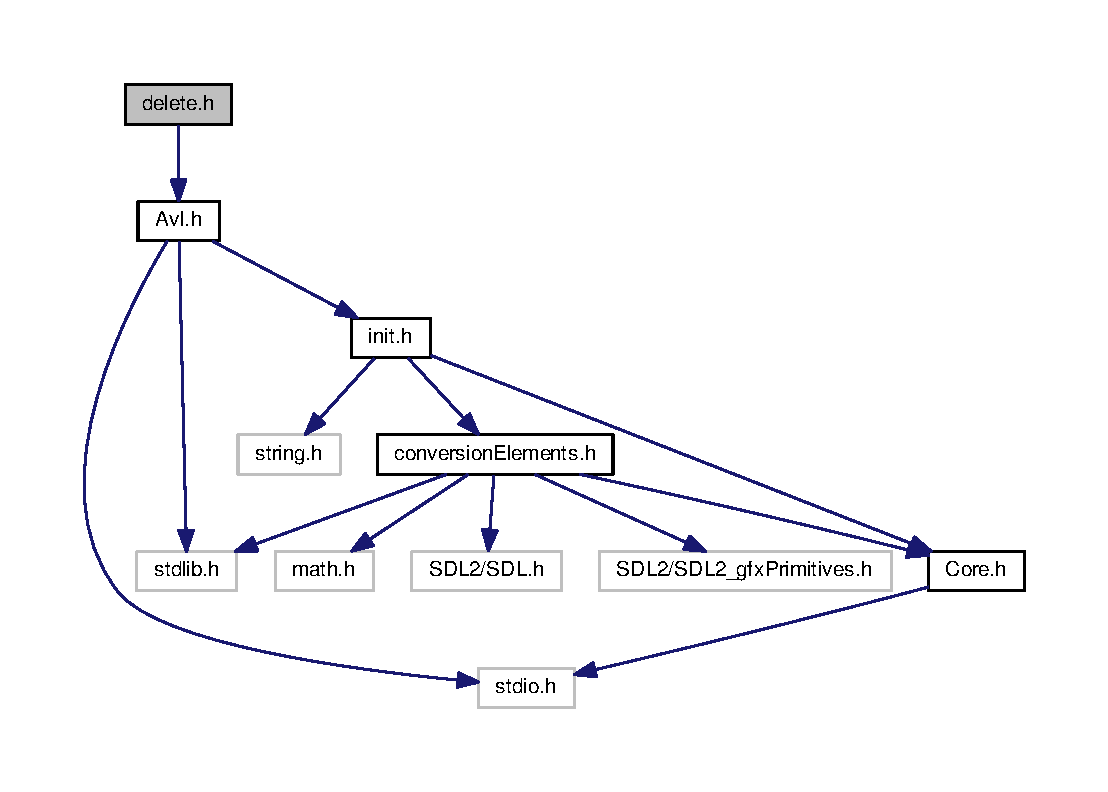
\includegraphics[width=350pt]{delete_8h__incl}
\end{center}
\end{figure}
This graph shows which files directly or indirectly include this file\-:
\nopagebreak
\begin{figure}[H]
\begin{center}
\leavevmode
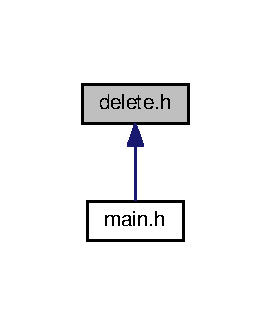
\includegraphics[width=130pt]{delete_8h__dep__incl}
\end{center}
\end{figure}
\subsection*{Functions}
\begin{DoxyCompactItemize}
\item 
void \hyperlink{delete_8h_ad754c1da05e433eeb224483438d6d5a7}{delete\-Coordinate} (\hyperlink{structCoordinate}{Coordinate} $\ast$c)
\item 
void \hyperlink{delete_8h_a4e05fb65ebbcd56d00e688e356a1351f}{delete\-Bounds} (\hyperlink{structBounds}{Bounds} $\ast$b)
\item 
void \hyperlink{delete_8h_a2054ef66b2a91686e692de6b86039390}{delete\-Color} (\hyperlink{structColor}{Color} $\ast$c)
\item 
void \hyperlink{delete_8h_a382f7ebaf756b41ba032b0e290b5f516}{delete\-Tag} (\hyperlink{structTag}{Tag} $\ast$t)
\item 
void \hyperlink{delete_8h_acb0f3666b83b4d008a67250e1cf83123}{delete\-Tab\-Tag} (\hyperlink{structTag}{Tag} $\ast$$\ast$t)
\item 
void \hyperlink{delete_8h_a3039fc4ca0a95e618defd345fb15c374}{delete\-Ref\-List\-Node} (\hyperlink{structrefListNode}{ref\-List\-Node} $\ast$r)
\item 
void \hyperlink{delete_8h_a20fcde4cd5c1832af41571eda7a3b354}{delete\-List\-Node} (\hyperlink{structListNode}{List\-Node} $\ast$l)
\item 
void \hyperlink{delete_8h_a00e184d58606e40ccadd140f1d558a78}{delete\-Ref\-List\-Way} (\hyperlink{structrefListWay}{ref\-List\-Way} $\ast$r)
\item 
void \hyperlink{delete_8h_abba7d9544581c9a16d37e95c65f1ffcd}{delete\-List\-Way} (\hyperlink{structListWay}{List\-Way} $\ast$l)
\item 
void \hyperlink{delete_8h_a8446cb9c727e0503ceaedaebe45855aa}{delete\-Ref\-List\-Rel} (\hyperlink{structrefListRel}{ref\-List\-Rel} $\ast$r)
\item 
void \hyperlink{delete_8h_afddcdba6a7fea86c3adaa74434cd9c4e}{delete\-List\-Relation} (\hyperlink{structListRelation}{List\-Relation} $\ast$l)
\item 
void \hyperlink{delete_8h_a10776a3abd69dfae7f75c7ce7cee3a69}{delete\-Node} (\hyperlink{structNode}{Node} $\ast$n)
\item 
void \hyperlink{delete_8h_a0aa33ed5aec66c1b0e0aae8327426b34}{delete\-Way} (\hyperlink{structWay}{Way} $\ast$w)
\item 
void \hyperlink{delete_8h_aa5df50b5d89c5cca564e35d0fdbea1aa}{delete\-Relation} (\hyperlink{structRelation}{Relation} $\ast$r)
\item 
void \hyperlink{delete_8h_a062b25ef0ead36d4cd7944abfe9494f9}{delete\-Avl} (\hyperlink{structAvl}{Avl} $\ast$$\ast$avl, int is\-Node)
\item 
void \hyperlink{delete_8h_af9a88755f0e56e50088c87ce1f89c58f}{delete\-Map} (\hyperlink{structMap}{Map} $\ast$map)
\end{DoxyCompactItemize}


\subsection{Detailed Description}
Initialisation of the principal structure. \begin{DoxyAuthor}{Author}
Isabelle M\-A\-R\-I\-N\-O Pierrick J\-A\-C\-Q\-U\-E\-T\-T\-E Hafça T\-I\-R\-I\-C\-H\-I\-N\-E 
\end{DoxyAuthor}
\begin{DoxyDate}{Date}
25 february 2016 
\end{DoxyDate}


\subsection{Function Documentation}
\hypertarget{delete_8h_a062b25ef0ead36d4cd7944abfe9494f9}{\index{delete.\-h@{delete.\-h}!delete\-Avl@{delete\-Avl}}
\index{delete\-Avl@{delete\-Avl}!delete.h@{delete.\-h}}
\subsubsection[{delete\-Avl}]{\setlength{\rightskip}{0pt plus 5cm}void delete\-Avl (
\begin{DoxyParamCaption}
\item[{{\bf Avl} $\ast$$\ast$}]{avl, }
\item[{int}]{is\-Node}
\end{DoxyParamCaption}
)}}\label{delete_8h_a062b25ef0ead36d4cd7944abfe9494f9}
Frees the memory of a avl 
\begin{DoxyParams}{Parameters}
{\em avl} & \hyperlink{structAvl}{Avl} which is deleted \\
\hline
\end{DoxyParams}


Here is the call graph for this function\-:
\nopagebreak
\begin{figure}[H]
\begin{center}
\leavevmode
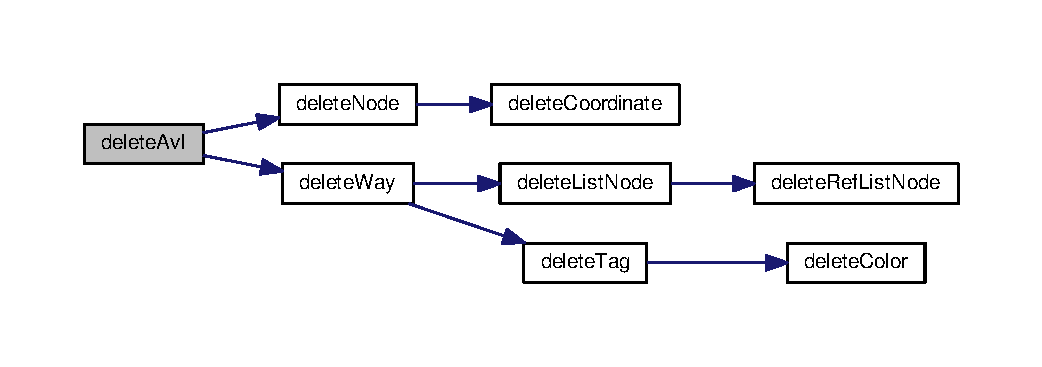
\includegraphics[width=350pt]{delete_8h_a062b25ef0ead36d4cd7944abfe9494f9_cgraph}
\end{center}
\end{figure}




Here is the caller graph for this function\-:
\nopagebreak
\begin{figure}[H]
\begin{center}
\leavevmode
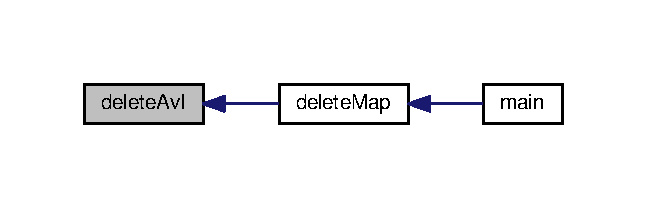
\includegraphics[width=310pt]{delete_8h_a062b25ef0ead36d4cd7944abfe9494f9_icgraph}
\end{center}
\end{figure}


\hypertarget{delete_8h_a4e05fb65ebbcd56d00e688e356a1351f}{\index{delete.\-h@{delete.\-h}!delete\-Bounds@{delete\-Bounds}}
\index{delete\-Bounds@{delete\-Bounds}!delete.h@{delete.\-h}}
\subsubsection[{delete\-Bounds}]{\setlength{\rightskip}{0pt plus 5cm}void delete\-Bounds (
\begin{DoxyParamCaption}
\item[{{\bf Bounds} $\ast$}]{b}
\end{DoxyParamCaption}
)}}\label{delete_8h_a4e05fb65ebbcd56d00e688e356a1351f}
Frees the memory of a \hyperlink{structBounds}{Bounds} 
\begin{DoxyParams}{Parameters}
{\em b} & \hyperlink{structBounds}{Bounds} which is deleted \\
\hline
\end{DoxyParams}


Here is the call graph for this function\-:
\nopagebreak
\begin{figure}[H]
\begin{center}
\leavevmode
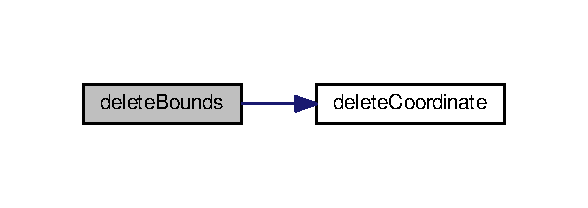
\includegraphics[width=282pt]{delete_8h_a4e05fb65ebbcd56d00e688e356a1351f_cgraph}
\end{center}
\end{figure}




Here is the caller graph for this function\-:
\nopagebreak
\begin{figure}[H]
\begin{center}
\leavevmode
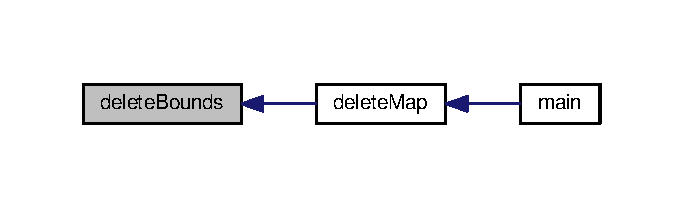
\includegraphics[width=328pt]{delete_8h_a4e05fb65ebbcd56d00e688e356a1351f_icgraph}
\end{center}
\end{figure}


\hypertarget{delete_8h_a2054ef66b2a91686e692de6b86039390}{\index{delete.\-h@{delete.\-h}!delete\-Color@{delete\-Color}}
\index{delete\-Color@{delete\-Color}!delete.h@{delete.\-h}}
\subsubsection[{delete\-Color}]{\setlength{\rightskip}{0pt plus 5cm}void delete\-Color (
\begin{DoxyParamCaption}
\item[{{\bf Color} $\ast$}]{c}
\end{DoxyParamCaption}
)}}\label{delete_8h_a2054ef66b2a91686e692de6b86039390}
Frees the memory of a \hyperlink{structColor}{Color} 
\begin{DoxyParams}{Parameters}
{\em c} & \hyperlink{structColor}{Color} which is deleted \\
\hline
\end{DoxyParams}


Here is the caller graph for this function\-:
\nopagebreak
\begin{figure}[H]
\begin{center}
\leavevmode
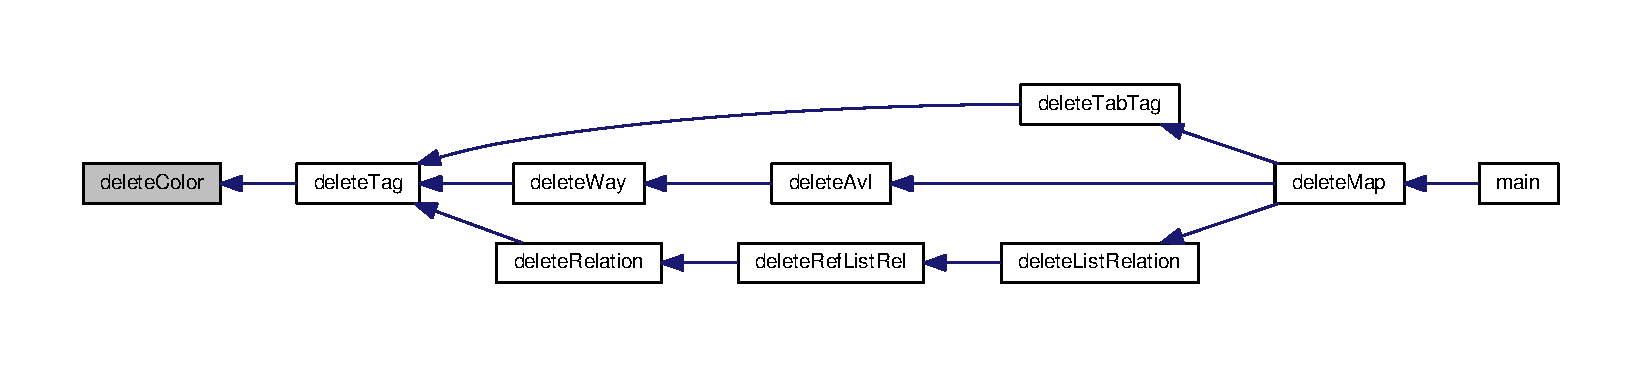
\includegraphics[width=350pt]{delete_8h_a2054ef66b2a91686e692de6b86039390_icgraph}
\end{center}
\end{figure}


\hypertarget{delete_8h_ad754c1da05e433eeb224483438d6d5a7}{\index{delete.\-h@{delete.\-h}!delete\-Coordinate@{delete\-Coordinate}}
\index{delete\-Coordinate@{delete\-Coordinate}!delete.h@{delete.\-h}}
\subsubsection[{delete\-Coordinate}]{\setlength{\rightskip}{0pt plus 5cm}void delete\-Coordinate (
\begin{DoxyParamCaption}
\item[{{\bf Coordinate} $\ast$}]{c}
\end{DoxyParamCaption}
)}}\label{delete_8h_ad754c1da05e433eeb224483438d6d5a7}
Frees the memory of a \hyperlink{structCoordinate}{Coordinate} 
\begin{DoxyParams}{Parameters}
{\em c} & \hyperlink{structCoordinate}{Coordinate} which is deleted \\
\hline
\end{DoxyParams}


Here is the caller graph for this function\-:
\nopagebreak
\begin{figure}[H]
\begin{center}
\leavevmode
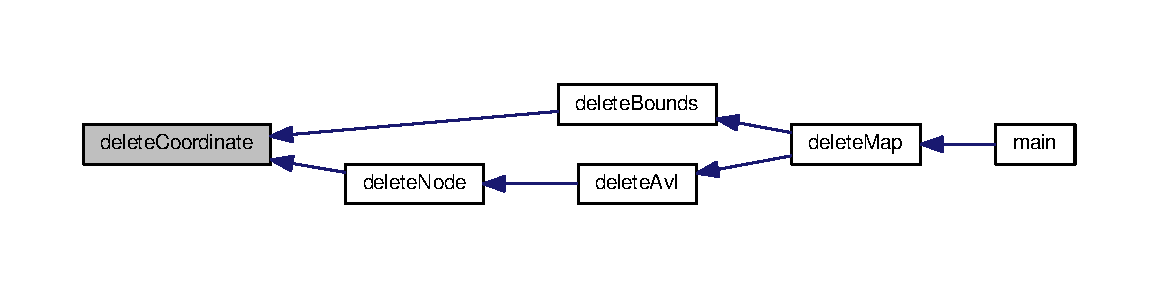
\includegraphics[width=350pt]{delete_8h_ad754c1da05e433eeb224483438d6d5a7_icgraph}
\end{center}
\end{figure}


\hypertarget{delete_8h_a20fcde4cd5c1832af41571eda7a3b354}{\index{delete.\-h@{delete.\-h}!delete\-List\-Node@{delete\-List\-Node}}
\index{delete\-List\-Node@{delete\-List\-Node}!delete.h@{delete.\-h}}
\subsubsection[{delete\-List\-Node}]{\setlength{\rightskip}{0pt plus 5cm}void delete\-List\-Node (
\begin{DoxyParamCaption}
\item[{{\bf List\-Node} $\ast$}]{l}
\end{DoxyParamCaption}
)}}\label{delete_8h_a20fcde4cd5c1832af41571eda7a3b354}
Frees the memory of a \hyperlink{structListNode}{List\-Node} 
\begin{DoxyParams}{Parameters}
{\em l} & \hyperlink{structListNode}{List\-Node} which is deleted \\
\hline
\end{DoxyParams}


Here is the call graph for this function\-:
\nopagebreak
\begin{figure}[H]
\begin{center}
\leavevmode
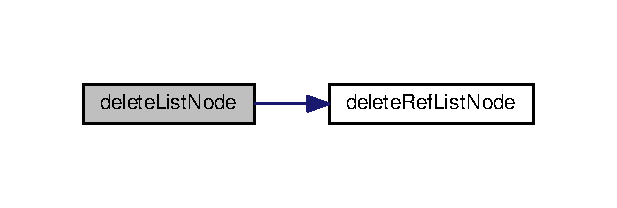
\includegraphics[width=296pt]{delete_8h_a20fcde4cd5c1832af41571eda7a3b354_cgraph}
\end{center}
\end{figure}




Here is the caller graph for this function\-:
\nopagebreak
\begin{figure}[H]
\begin{center}
\leavevmode
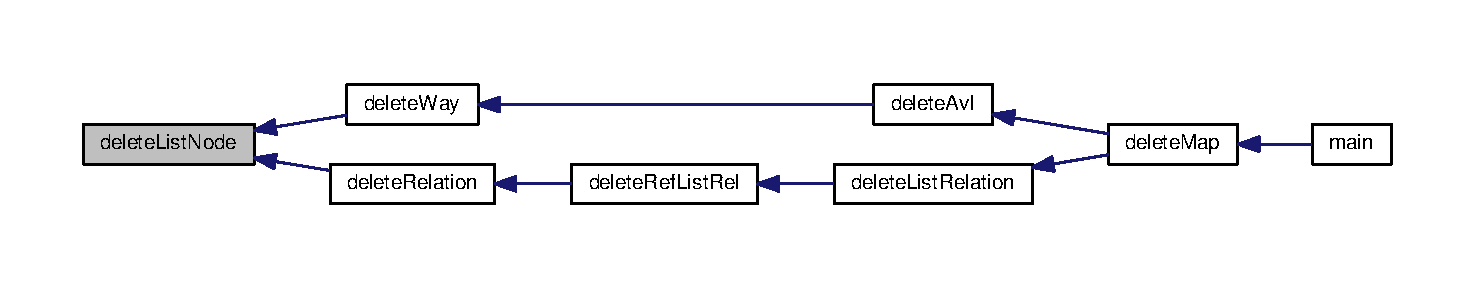
\includegraphics[width=350pt]{delete_8h_a20fcde4cd5c1832af41571eda7a3b354_icgraph}
\end{center}
\end{figure}


\hypertarget{delete_8h_afddcdba6a7fea86c3adaa74434cd9c4e}{\index{delete.\-h@{delete.\-h}!delete\-List\-Relation@{delete\-List\-Relation}}
\index{delete\-List\-Relation@{delete\-List\-Relation}!delete.h@{delete.\-h}}
\subsubsection[{delete\-List\-Relation}]{\setlength{\rightskip}{0pt plus 5cm}void delete\-List\-Relation (
\begin{DoxyParamCaption}
\item[{{\bf List\-Relation} $\ast$}]{l}
\end{DoxyParamCaption}
)}}\label{delete_8h_afddcdba6a7fea86c3adaa74434cd9c4e}
Frees the memory of a \hyperlink{structListRelation}{List\-Relation} 
\begin{DoxyParams}{Parameters}
{\em l} & \hyperlink{structListRelation}{List\-Relation} which is deleted \\
\hline
\end{DoxyParams}


Here is the call graph for this function\-:
\nopagebreak
\begin{figure}[H]
\begin{center}
\leavevmode
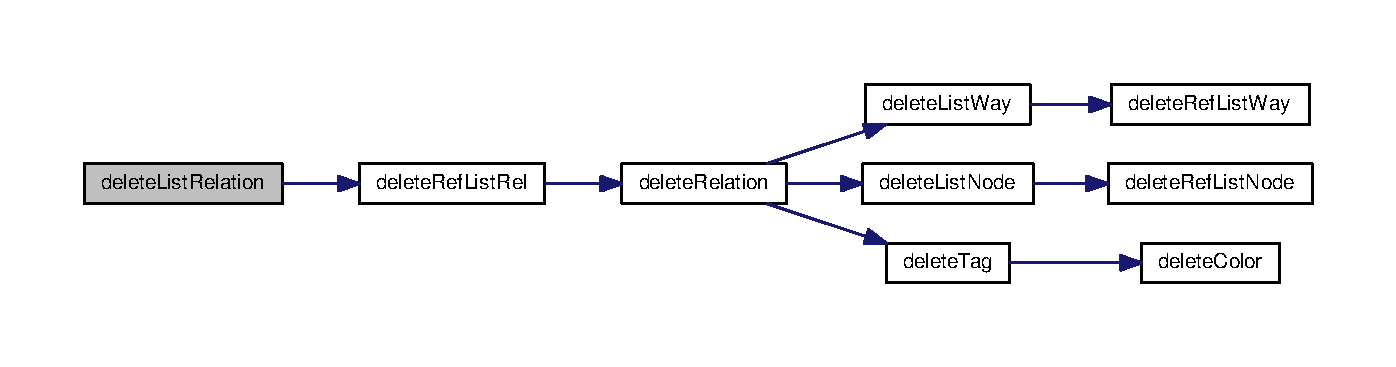
\includegraphics[width=350pt]{delete_8h_afddcdba6a7fea86c3adaa74434cd9c4e_cgraph}
\end{center}
\end{figure}




Here is the caller graph for this function\-:
\nopagebreak
\begin{figure}[H]
\begin{center}
\leavevmode
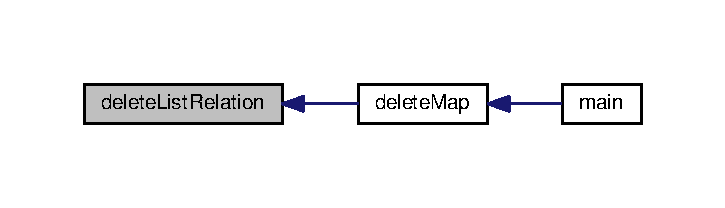
\includegraphics[width=348pt]{delete_8h_afddcdba6a7fea86c3adaa74434cd9c4e_icgraph}
\end{center}
\end{figure}


\hypertarget{delete_8h_abba7d9544581c9a16d37e95c65f1ffcd}{\index{delete.\-h@{delete.\-h}!delete\-List\-Way@{delete\-List\-Way}}
\index{delete\-List\-Way@{delete\-List\-Way}!delete.h@{delete.\-h}}
\subsubsection[{delete\-List\-Way}]{\setlength{\rightskip}{0pt plus 5cm}void delete\-List\-Way (
\begin{DoxyParamCaption}
\item[{{\bf List\-Way} $\ast$}]{l}
\end{DoxyParamCaption}
)}}\label{delete_8h_abba7d9544581c9a16d37e95c65f1ffcd}
Frees the memory of a \hyperlink{structListWay}{List\-Way} 
\begin{DoxyParams}{Parameters}
{\em l} & \hyperlink{structListWay}{List\-Way} which is deleted \\
\hline
\end{DoxyParams}


Here is the call graph for this function\-:
\nopagebreak
\begin{figure}[H]
\begin{center}
\leavevmode
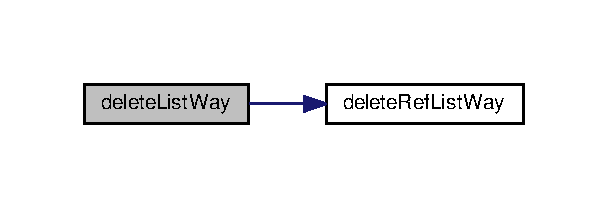
\includegraphics[width=292pt]{delete_8h_abba7d9544581c9a16d37e95c65f1ffcd_cgraph}
\end{center}
\end{figure}




Here is the caller graph for this function\-:
\nopagebreak
\begin{figure}[H]
\begin{center}
\leavevmode
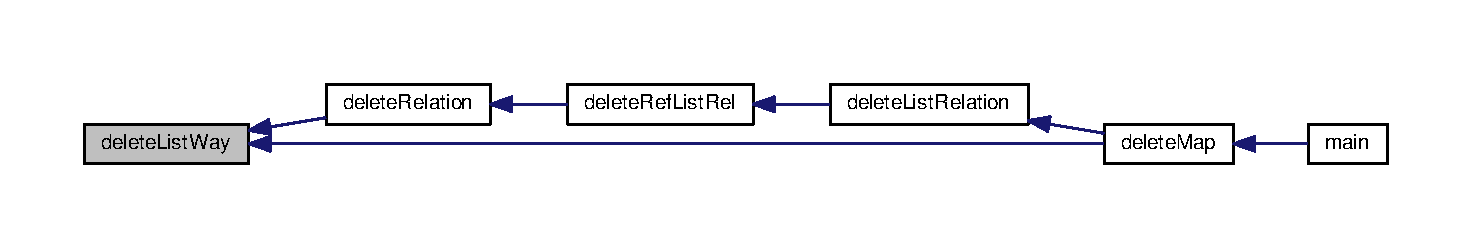
\includegraphics[width=350pt]{delete_8h_abba7d9544581c9a16d37e95c65f1ffcd_icgraph}
\end{center}
\end{figure}


\hypertarget{delete_8h_af9a88755f0e56e50088c87ce1f89c58f}{\index{delete.\-h@{delete.\-h}!delete\-Map@{delete\-Map}}
\index{delete\-Map@{delete\-Map}!delete.h@{delete.\-h}}
\subsubsection[{delete\-Map}]{\setlength{\rightskip}{0pt plus 5cm}void delete\-Map (
\begin{DoxyParamCaption}
\item[{{\bf Map} $\ast$}]{map}
\end{DoxyParamCaption}
)}}\label{delete_8h_af9a88755f0e56e50088c87ce1f89c58f}
Frees the memory of a \hyperlink{structMap}{Map} 
\begin{DoxyParams}{Parameters}
{\em \hyperlink{structMap}{Map}} & which is deleted \\
\hline
\end{DoxyParams}


Here is the call graph for this function\-:
\nopagebreak
\begin{figure}[H]
\begin{center}
\leavevmode
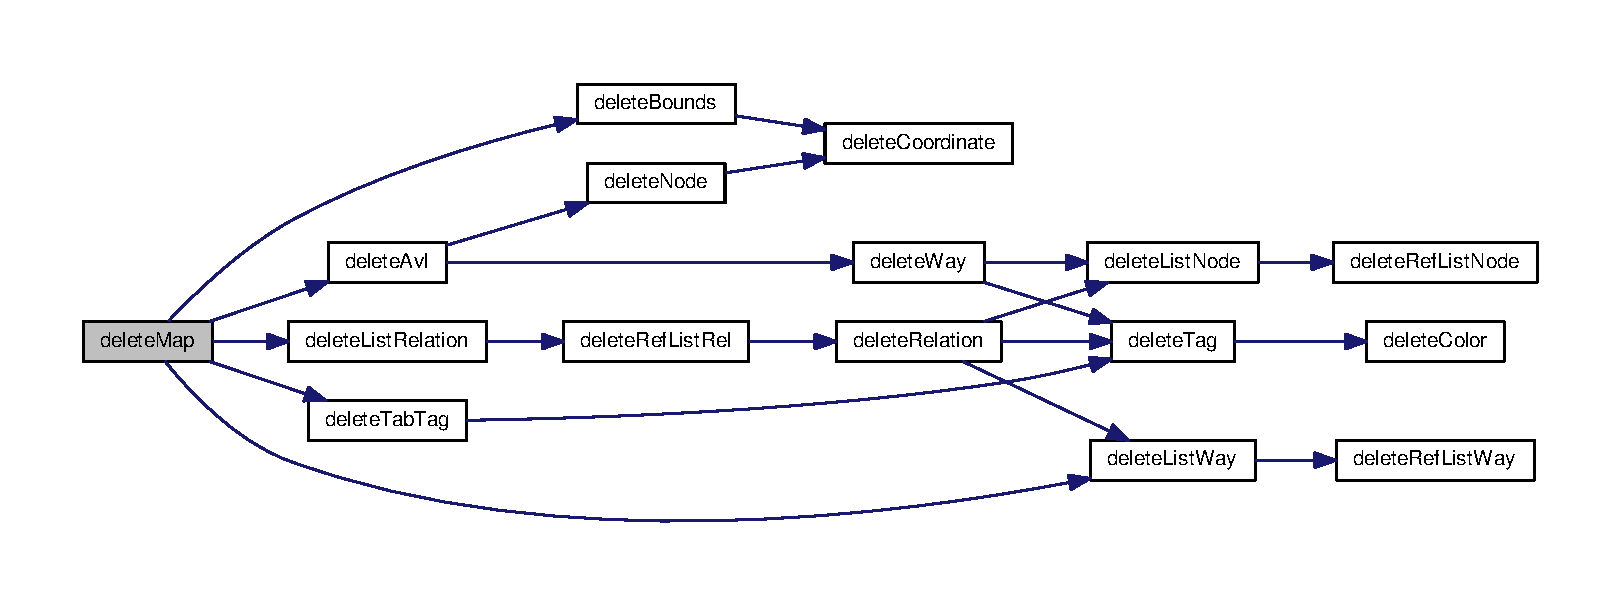
\includegraphics[width=350pt]{delete_8h_af9a88755f0e56e50088c87ce1f89c58f_cgraph}
\end{center}
\end{figure}




Here is the caller graph for this function\-:
\nopagebreak
\begin{figure}[H]
\begin{center}
\leavevmode
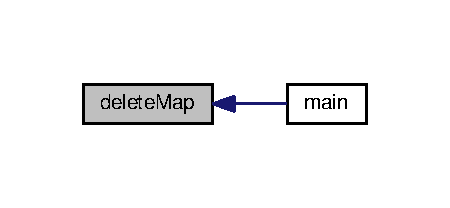
\includegraphics[width=216pt]{delete_8h_af9a88755f0e56e50088c87ce1f89c58f_icgraph}
\end{center}
\end{figure}


\hypertarget{delete_8h_a10776a3abd69dfae7f75c7ce7cee3a69}{\index{delete.\-h@{delete.\-h}!delete\-Node@{delete\-Node}}
\index{delete\-Node@{delete\-Node}!delete.h@{delete.\-h}}
\subsubsection[{delete\-Node}]{\setlength{\rightskip}{0pt plus 5cm}void delete\-Node (
\begin{DoxyParamCaption}
\item[{{\bf Node} $\ast$}]{n}
\end{DoxyParamCaption}
)}}\label{delete_8h_a10776a3abd69dfae7f75c7ce7cee3a69}
Frees the memory of a \hyperlink{structNode}{Node} 
\begin{DoxyParams}{Parameters}
{\em n} & \hyperlink{structNode}{Node} which is deleted \\
\hline
\end{DoxyParams}


Here is the call graph for this function\-:
\nopagebreak
\begin{figure}[H]
\begin{center}
\leavevmode
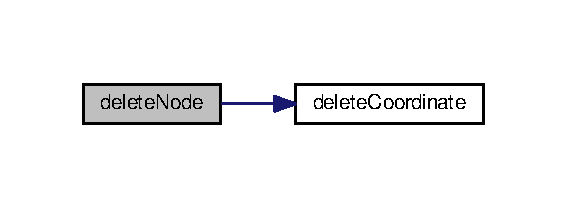
\includegraphics[width=272pt]{delete_8h_a10776a3abd69dfae7f75c7ce7cee3a69_cgraph}
\end{center}
\end{figure}




Here is the caller graph for this function\-:
\nopagebreak
\begin{figure}[H]
\begin{center}
\leavevmode
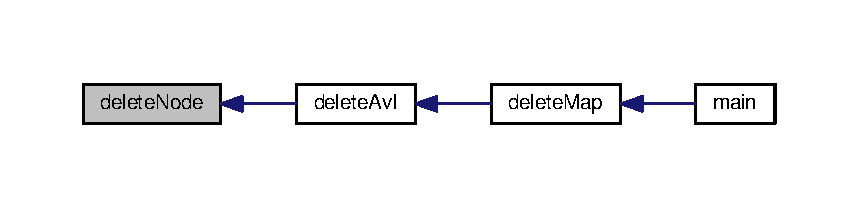
\includegraphics[width=350pt]{delete_8h_a10776a3abd69dfae7f75c7ce7cee3a69_icgraph}
\end{center}
\end{figure}


\hypertarget{delete_8h_a3039fc4ca0a95e618defd345fb15c374}{\index{delete.\-h@{delete.\-h}!delete\-Ref\-List\-Node@{delete\-Ref\-List\-Node}}
\index{delete\-Ref\-List\-Node@{delete\-Ref\-List\-Node}!delete.h@{delete.\-h}}
\subsubsection[{delete\-Ref\-List\-Node}]{\setlength{\rightskip}{0pt plus 5cm}void delete\-Ref\-List\-Node (
\begin{DoxyParamCaption}
\item[{{\bf ref\-List\-Node} $\ast$}]{r}
\end{DoxyParamCaption}
)}}\label{delete_8h_a3039fc4ca0a95e618defd345fb15c374}
Frees the memory of a Ref\-List\-Node 
\begin{DoxyParams}{Parameters}
{\em r} & Ref\-List\-Node which is deleted \\
\hline
\end{DoxyParams}


Here is the caller graph for this function\-:
\nopagebreak
\begin{figure}[H]
\begin{center}
\leavevmode
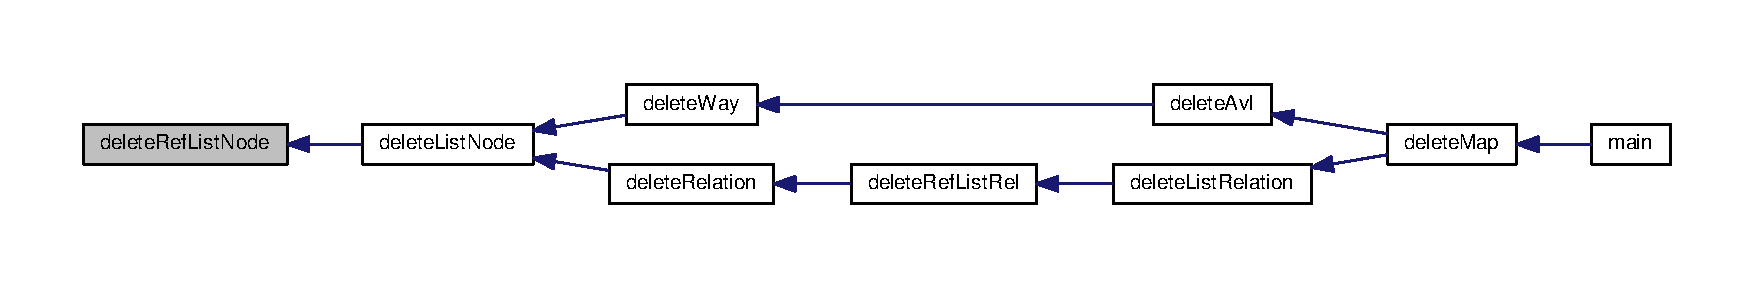
\includegraphics[width=350pt]{delete_8h_a3039fc4ca0a95e618defd345fb15c374_icgraph}
\end{center}
\end{figure}


\hypertarget{delete_8h_a8446cb9c727e0503ceaedaebe45855aa}{\index{delete.\-h@{delete.\-h}!delete\-Ref\-List\-Rel@{delete\-Ref\-List\-Rel}}
\index{delete\-Ref\-List\-Rel@{delete\-Ref\-List\-Rel}!delete.h@{delete.\-h}}
\subsubsection[{delete\-Ref\-List\-Rel}]{\setlength{\rightskip}{0pt plus 5cm}void delete\-Ref\-List\-Rel (
\begin{DoxyParamCaption}
\item[{{\bf ref\-List\-Rel} $\ast$}]{r}
\end{DoxyParamCaption}
)}}\label{delete_8h_a8446cb9c727e0503ceaedaebe45855aa}
Frees the memory of a \hyperlink{structrefListRel}{ref\-List\-Rel} 
\begin{DoxyParams}{Parameters}
{\em r} & \hyperlink{structrefListRel}{ref\-List\-Rel} which is deleted \\
\hline
\end{DoxyParams}


Here is the call graph for this function\-:
\nopagebreak
\begin{figure}[H]
\begin{center}
\leavevmode
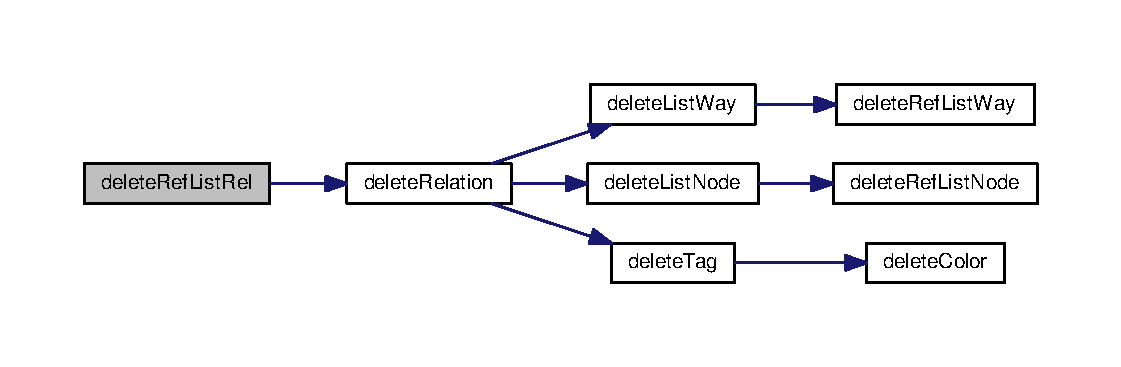
\includegraphics[width=350pt]{delete_8h_a8446cb9c727e0503ceaedaebe45855aa_cgraph}
\end{center}
\end{figure}




Here is the caller graph for this function\-:
\nopagebreak
\begin{figure}[H]
\begin{center}
\leavevmode
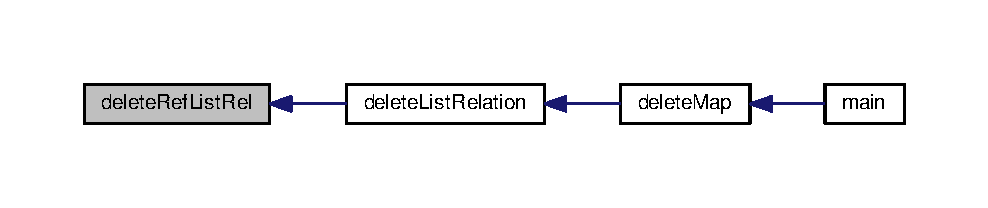
\includegraphics[width=350pt]{delete_8h_a8446cb9c727e0503ceaedaebe45855aa_icgraph}
\end{center}
\end{figure}


\hypertarget{delete_8h_a00e184d58606e40ccadd140f1d558a78}{\index{delete.\-h@{delete.\-h}!delete\-Ref\-List\-Way@{delete\-Ref\-List\-Way}}
\index{delete\-Ref\-List\-Way@{delete\-Ref\-List\-Way}!delete.h@{delete.\-h}}
\subsubsection[{delete\-Ref\-List\-Way}]{\setlength{\rightskip}{0pt plus 5cm}void delete\-Ref\-List\-Way (
\begin{DoxyParamCaption}
\item[{{\bf ref\-List\-Way} $\ast$}]{r}
\end{DoxyParamCaption}
)}}\label{delete_8h_a00e184d58606e40ccadd140f1d558a78}
Frees the memory of a \hyperlink{structrefListWay}{ref\-List\-Way} 
\begin{DoxyParams}{Parameters}
{\em r} & \hyperlink{structrefListWay}{ref\-List\-Way} which is deleted \\
\hline
\end{DoxyParams}


Here is the caller graph for this function\-:
\nopagebreak
\begin{figure}[H]
\begin{center}
\leavevmode
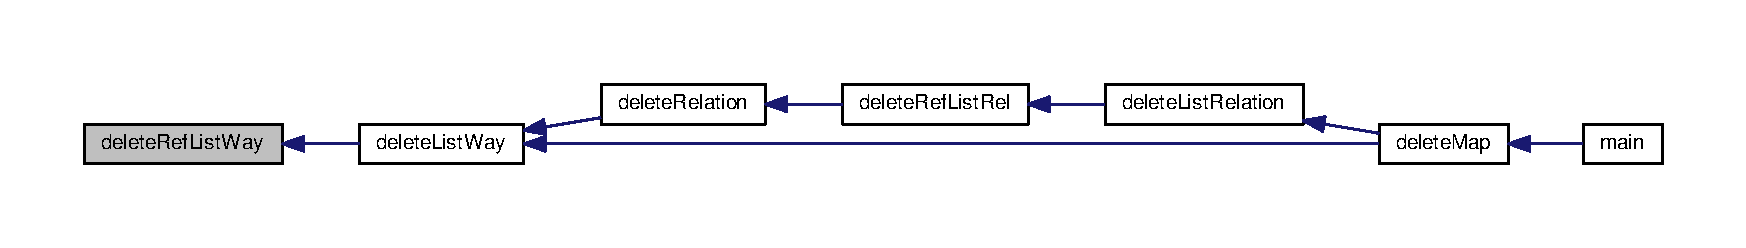
\includegraphics[width=350pt]{delete_8h_a00e184d58606e40ccadd140f1d558a78_icgraph}
\end{center}
\end{figure}


\hypertarget{delete_8h_aa5df50b5d89c5cca564e35d0fdbea1aa}{\index{delete.\-h@{delete.\-h}!delete\-Relation@{delete\-Relation}}
\index{delete\-Relation@{delete\-Relation}!delete.h@{delete.\-h}}
\subsubsection[{delete\-Relation}]{\setlength{\rightskip}{0pt plus 5cm}void delete\-Relation (
\begin{DoxyParamCaption}
\item[{{\bf Relation} $\ast$}]{r}
\end{DoxyParamCaption}
)}}\label{delete_8h_aa5df50b5d89c5cca564e35d0fdbea1aa}
Frees the memory of a \hyperlink{structRelation}{Relation} 
\begin{DoxyParams}{Parameters}
{\em r} & \hyperlink{structRelation}{Relation} which is deleted \\
\hline
\end{DoxyParams}


Here is the call graph for this function\-:
\nopagebreak
\begin{figure}[H]
\begin{center}
\leavevmode
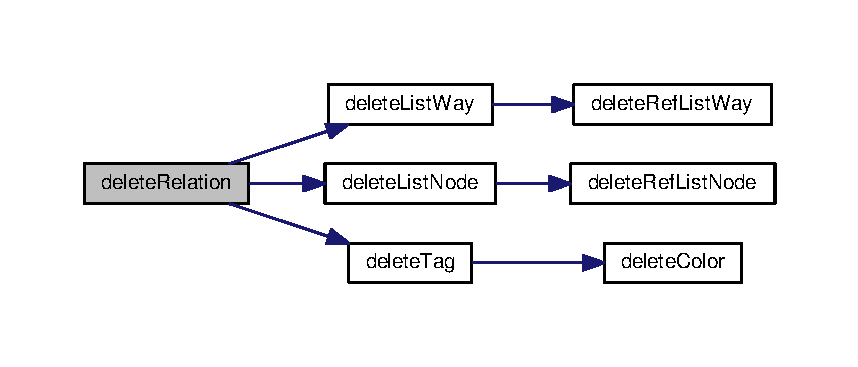
\includegraphics[width=350pt]{delete_8h_aa5df50b5d89c5cca564e35d0fdbea1aa_cgraph}
\end{center}
\end{figure}




Here is the caller graph for this function\-:
\nopagebreak
\begin{figure}[H]
\begin{center}
\leavevmode
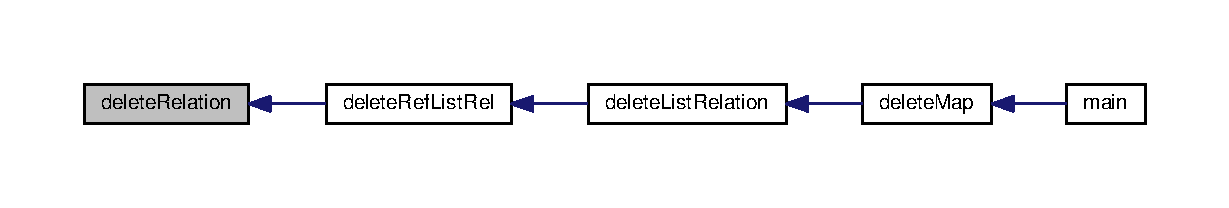
\includegraphics[width=350pt]{delete_8h_aa5df50b5d89c5cca564e35d0fdbea1aa_icgraph}
\end{center}
\end{figure}


\hypertarget{delete_8h_acb0f3666b83b4d008a67250e1cf83123}{\index{delete.\-h@{delete.\-h}!delete\-Tab\-Tag@{delete\-Tab\-Tag}}
\index{delete\-Tab\-Tag@{delete\-Tab\-Tag}!delete.h@{delete.\-h}}
\subsubsection[{delete\-Tab\-Tag}]{\setlength{\rightskip}{0pt plus 5cm}void delete\-Tab\-Tag (
\begin{DoxyParamCaption}
\item[{{\bf Tag} $\ast$$\ast$}]{t}
\end{DoxyParamCaption}
)}}\label{delete_8h_acb0f3666b83b4d008a67250e1cf83123}
Frees the memory of a Tab\-Tag 
\begin{DoxyParams}{Parameters}
{\em t} & \hyperlink{structTag}{Tag} which is deleted \\
\hline
\end{DoxyParams}


Here is the call graph for this function\-:
\nopagebreak
\begin{figure}[H]
\begin{center}
\leavevmode
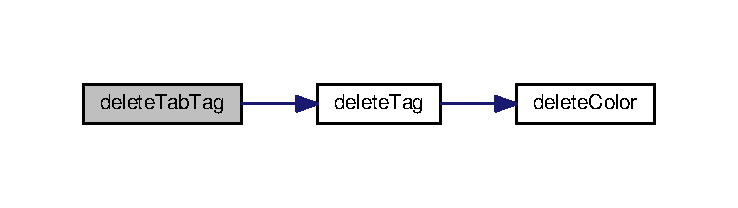
\includegraphics[width=350pt]{delete_8h_acb0f3666b83b4d008a67250e1cf83123_cgraph}
\end{center}
\end{figure}




Here is the caller graph for this function\-:
\nopagebreak
\begin{figure}[H]
\begin{center}
\leavevmode
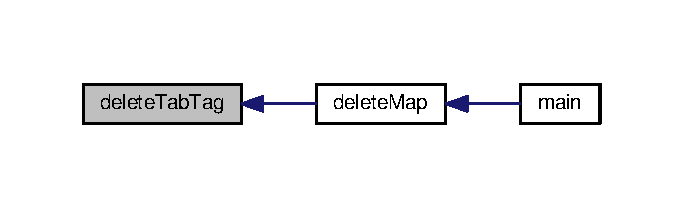
\includegraphics[width=328pt]{delete_8h_acb0f3666b83b4d008a67250e1cf83123_icgraph}
\end{center}
\end{figure}


\hypertarget{delete_8h_a382f7ebaf756b41ba032b0e290b5f516}{\index{delete.\-h@{delete.\-h}!delete\-Tag@{delete\-Tag}}
\index{delete\-Tag@{delete\-Tag}!delete.h@{delete.\-h}}
\subsubsection[{delete\-Tag}]{\setlength{\rightskip}{0pt plus 5cm}void delete\-Tag (
\begin{DoxyParamCaption}
\item[{{\bf Tag} $\ast$}]{t}
\end{DoxyParamCaption}
)}}\label{delete_8h_a382f7ebaf756b41ba032b0e290b5f516}
Frees the memory of a \hyperlink{structTag}{Tag} 
\begin{DoxyParams}{Parameters}
{\em t} & \hyperlink{structTag}{Tag} which is deleted \\
\hline
\end{DoxyParams}


Here is the call graph for this function\-:
\nopagebreak
\begin{figure}[H]
\begin{center}
\leavevmode
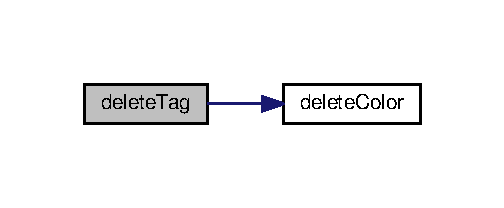
\includegraphics[width=242pt]{delete_8h_a382f7ebaf756b41ba032b0e290b5f516_cgraph}
\end{center}
\end{figure}




Here is the caller graph for this function\-:
\nopagebreak
\begin{figure}[H]
\begin{center}
\leavevmode
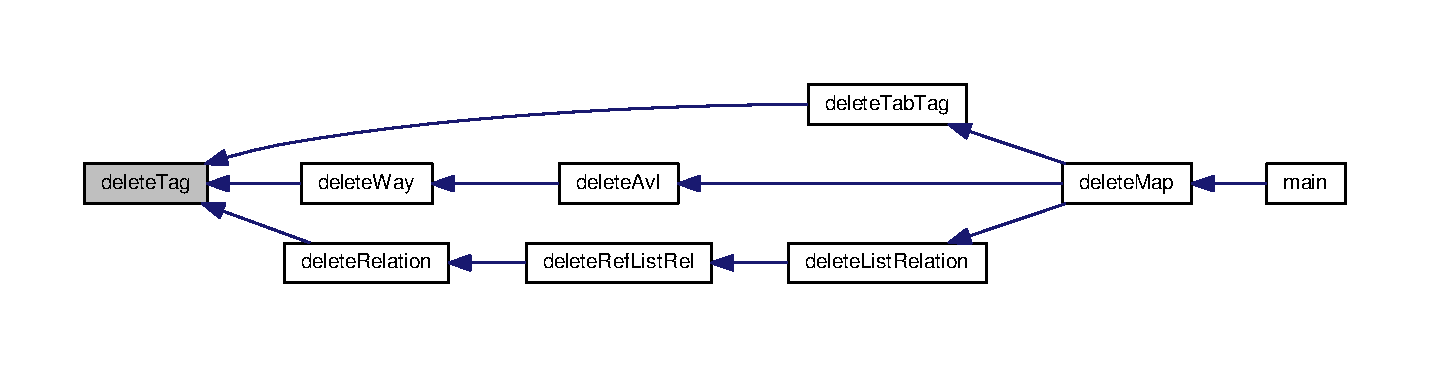
\includegraphics[width=350pt]{delete_8h_a382f7ebaf756b41ba032b0e290b5f516_icgraph}
\end{center}
\end{figure}


\hypertarget{delete_8h_a0aa33ed5aec66c1b0e0aae8327426b34}{\index{delete.\-h@{delete.\-h}!delete\-Way@{delete\-Way}}
\index{delete\-Way@{delete\-Way}!delete.h@{delete.\-h}}
\subsubsection[{delete\-Way}]{\setlength{\rightskip}{0pt plus 5cm}void delete\-Way (
\begin{DoxyParamCaption}
\item[{{\bf Way} $\ast$}]{w}
\end{DoxyParamCaption}
)}}\label{delete_8h_a0aa33ed5aec66c1b0e0aae8327426b34}
Frees the memory of a \hyperlink{structWay}{Way} 
\begin{DoxyParams}{Parameters}
{\em w} & \hyperlink{structWay}{Way} which is deleted \\
\hline
\end{DoxyParams}


Here is the call graph for this function\-:
\nopagebreak
\begin{figure}[H]
\begin{center}
\leavevmode
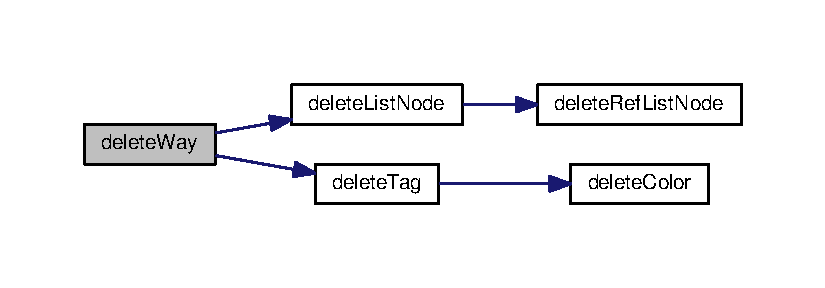
\includegraphics[width=350pt]{delete_8h_a0aa33ed5aec66c1b0e0aae8327426b34_cgraph}
\end{center}
\end{figure}




Here is the caller graph for this function\-:
\nopagebreak
\begin{figure}[H]
\begin{center}
\leavevmode
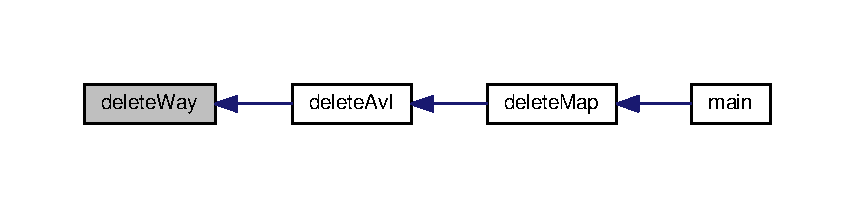
\includegraphics[width=350pt]{delete_8h_a0aa33ed5aec66c1b0e0aae8327426b34_icgraph}
\end{center}
\end{figure}



\hypertarget{evenement_8h}{\section{evenement.\-h File Reference}
\label{evenement_8h}\index{evenement.\-h@{evenement.\-h}}
}


Declare fonctions to convert elements.  


{\ttfamily \#include \char`\"{}point.\-h\char`\"{}}\\*
{\ttfamily \#include \char`\"{}line.\-h\char`\"{}}\\*
Include dependency graph for evenement.\-h\-:
\nopagebreak
\begin{figure}[H]
\begin{center}
\leavevmode
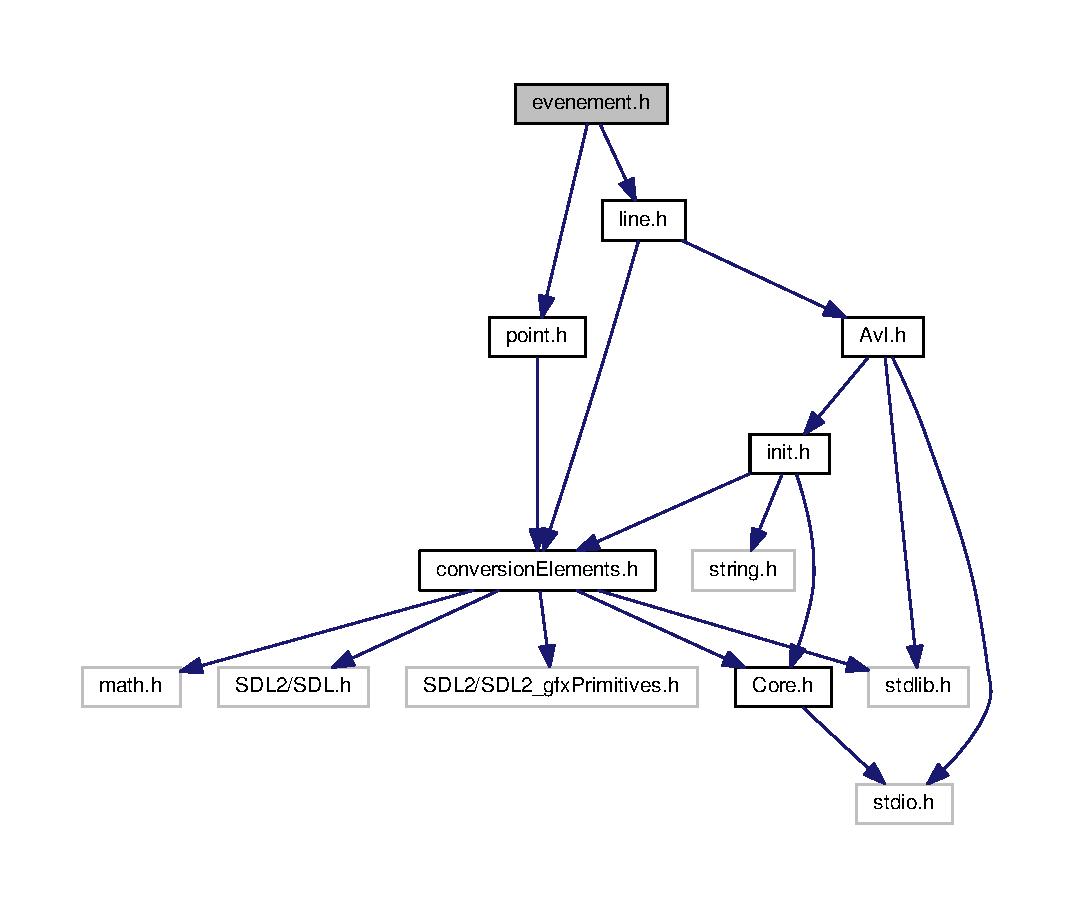
\includegraphics[width=350pt]{evenement_8h__incl}
\end{center}
\end{figure}
This graph shows which files directly or indirectly include this file\-:
\nopagebreak
\begin{figure}[H]
\begin{center}
\leavevmode
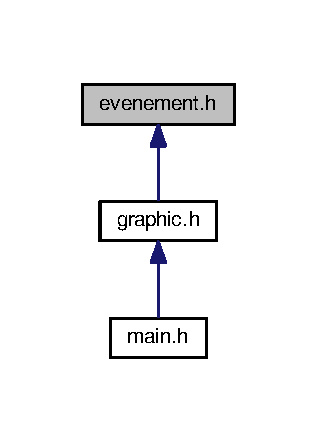
\includegraphics[width=152pt]{evenement_8h__dep__incl}
\end{center}
\end{figure}
\subsection*{Functions}
\begin{DoxyCompactItemize}
\item 
void \hyperlink{evenement_8h_a992ddeca01850c361d0baaae2d2e206f}{evenement} ()
\item 
void \hyperlink{evenement_8h_a96c334a614da0507d23f49d2c23e062b}{draw\-Map} (\hyperlink{structMap}{Map} $\ast$m, char $\ast$type\-Of\-Dessin)
\end{DoxyCompactItemize}
\subsection*{Variables}
\begin{DoxyCompactItemize}
\item 
\hypertarget{evenement_8h_a076489b58a3cd509b38f120ae469da1b}{char $\ast$ {\bfseries type\-Of\-Draw}}\label{evenement_8h_a076489b58a3cd509b38f120ae469da1b}

\end{DoxyCompactItemize}


\subsection{Detailed Description}
Declare fonctions to convert elements. \begin{DoxyAuthor}{Author}
Isabelle M\-A\-R\-I\-N\-O Pierrick J\-A\-C\-Q\-U\-E\-T\-T\-E Hafça T\-I\-R\-I\-C\-H\-I\-N\-E 
\end{DoxyAuthor}
\begin{DoxyDate}{Date}
8 April 2016
\end{DoxyDate}
Evenement Window 

\subsection{Function Documentation}
\hypertarget{evenement_8h_a96c334a614da0507d23f49d2c23e062b}{\index{evenement.\-h@{evenement.\-h}!draw\-Map@{draw\-Map}}
\index{draw\-Map@{draw\-Map}!evenement.h@{evenement.\-h}}
\subsubsection[{draw\-Map}]{\setlength{\rightskip}{0pt plus 5cm}void draw\-Map (
\begin{DoxyParamCaption}
\item[{{\bf Map} $\ast$}]{m, }
\item[{char $\ast$}]{type\-Of\-Dessin}
\end{DoxyParamCaption}
)}}\label{evenement_8h_a96c334a614da0507d23f49d2c23e062b}
Fonction that browse the avl tree by calling the \char`\"{}parcours\-Avl\char`\"{} fonction and displays it to the screen by calling the \char`\"{}evenement\char`\"{} fonction 
\begin{DoxyParams}{Parameters}
{\em Map$\ast$} & is the pointer to the information of map \\
\hline
{\em $\ast$type\-Of\-Dessin} & is the line or ponct \\
\hline
\end{DoxyParams}


Here is the caller graph for this function\-:
\nopagebreak
\begin{figure}[H]
\begin{center}
\leavevmode
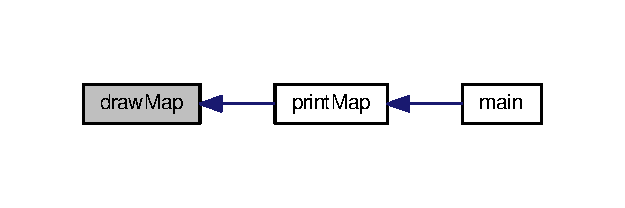
\includegraphics[width=300pt]{evenement_8h_a96c334a614da0507d23f49d2c23e062b_icgraph}
\end{center}
\end{figure}


\hypertarget{evenement_8h_a992ddeca01850c361d0baaae2d2e206f}{\index{evenement.\-h@{evenement.\-h}!evenement@{evenement}}
\index{evenement@{evenement}!evenement.h@{evenement.\-h}}
\subsubsection[{evenement}]{\setlength{\rightskip}{0pt plus 5cm}void evenement (
\begin{DoxyParamCaption}
{}
\end{DoxyParamCaption}
)}}\label{evenement_8h_a992ddeca01850c361d0baaae2d2e206f}
Fonction that permit the display While we haven't closed the window it is still on the screen When we do close it, it displays a message saying we closed it This event is handeled by a loop \-: while the statut is \char`\"{}\-C\-O\-N\-T\-I\-N\-U\-E\char`\"{} we keep the window to the screen Otherwise, we close it and change the statut to \char`\"{}\-Q\-U\-I\-T\char`\"{} 

Here is the call graph for this function\-:
\nopagebreak
\begin{figure}[H]
\begin{center}
\leavevmode
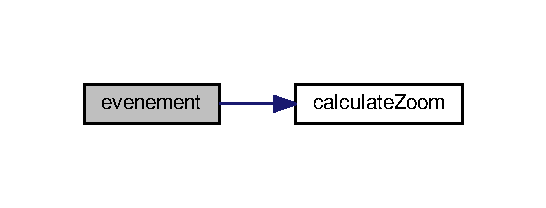
\includegraphics[width=262pt]{evenement_8h_a992ddeca01850c361d0baaae2d2e206f_cgraph}
\end{center}
\end{figure}




Here is the caller graph for this function\-:
\nopagebreak
\begin{figure}[H]
\begin{center}
\leavevmode
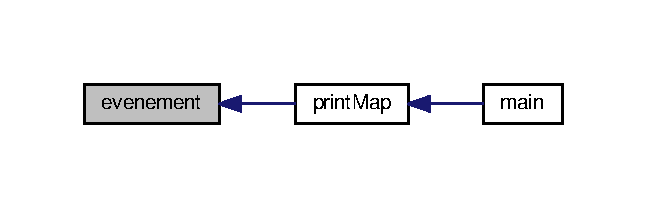
\includegraphics[width=310pt]{evenement_8h_a992ddeca01850c361d0baaae2d2e206f_icgraph}
\end{center}
\end{figure}



\hypertarget{graphic_8h}{\section{graphic.\-h File Reference}
\label{graphic_8h}\index{graphic.\-h@{graphic.\-h}}
}


Display the \hyperlink{structNode}{Node} and the way from a map.  


{\ttfamily \#include \char`\"{}evenement.\-h\char`\"{}}\\*
Include dependency graph for graphic.\-h\-:
\nopagebreak
\begin{figure}[H]
\begin{center}
\leavevmode
\includegraphics[width=350pt]{graphic_8h__incl}
\end{center}
\end{figure}
This graph shows which files directly or indirectly include this file\-:
\nopagebreak
\begin{figure}[H]
\begin{center}
\leavevmode
\includegraphics[width=134pt]{graphic_8h__dep__incl}
\end{center}
\end{figure}
\subsection*{Functions}
\begin{DoxyCompactItemize}
\item 
void \hyperlink{graphic_8h_a93642d42e7cad3d6ee5cd6d0e719e127}{print\-Map} (\hyperlink{structMap}{Map} $\ast$map, char $\ast$type\-Of\-Dessin, char $\ast$signal)
\end{DoxyCompactItemize}


\subsection{Detailed Description}
Display the \hyperlink{structNode}{Node} and the way from a map. \begin{DoxyAuthor}{Author}
Isabelle M\-A\-R\-I\-N\-O Pierrick J\-A\-C\-Q\-U\-E\-T\-T\-E Hafça T\-I\-R\-I\-C\-H\-I\-N\-E 
\end{DoxyAuthor}
\begin{DoxyDate}{Date}
20 april 2016 
\end{DoxyDate}


\subsection{Function Documentation}
\hypertarget{graphic_8h_a93642d42e7cad3d6ee5cd6d0e719e127}{\index{graphic.\-h@{graphic.\-h}!print\-Map@{print\-Map}}
\index{print\-Map@{print\-Map}!graphic.h@{graphic.\-h}}
\subsubsection[{print\-Map}]{\setlength{\rightskip}{0pt plus 5cm}void print\-Map (
\begin{DoxyParamCaption}
\item[{{\bf Map} $\ast$}]{map, }
\item[{char $\ast$}]{type\-Of\-Dessin, }
\item[{char $\ast$}]{signal}
\end{DoxyParamCaption}
)}}\label{graphic_8h_a93642d42e7cad3d6ee5cd6d0e719e127}
Fonction that creates a window with the right scales 
\begin{DoxyParams}{Parameters}
{\em Map$\ast$} & is the pointer to the information of map \\
\hline
{\em char$\ast$} & type\-Of\-Dessin is the line or ponct \\
\hline
{\em char$\ast$} & signal is the optional signal to know when the map is all printed \\
\hline
\end{DoxyParams}


Here is the call graph for this function\-:
\nopagebreak
\begin{figure}[H]
\begin{center}
\leavevmode
\includegraphics[width=350pt]{graphic_8h_a93642d42e7cad3d6ee5cd6d0e719e127_cgraph}
\end{center}
\end{figure}




Here is the caller graph for this function\-:
\nopagebreak
\begin{figure}[H]
\begin{center}
\leavevmode
\includegraphics[width=208pt]{graphic_8h_a93642d42e7cad3d6ee5cd6d0e719e127_icgraph}
\end{center}
\end{figure}



\hypertarget{init_8h}{\section{init.\-h File Reference}
\label{init_8h}\index{init.\-h@{init.\-h}}
}


Initialisation of the principal structure.  


{\ttfamily \#include $<$string.\-h$>$}\\*
{\ttfamily \#include \char`\"{}conversion\-Elements.\-h\char`\"{}}\\*
Include dependency graph for init.\-h\-:
\nopagebreak
\begin{figure}[H]
\begin{center}
\leavevmode
\includegraphics[width=350pt]{init_8h__incl}
\end{center}
\end{figure}
This graph shows which files directly or indirectly include this file\-:
\nopagebreak
\begin{figure}[H]
\begin{center}
\leavevmode
\includegraphics[width=279pt]{init_8h__dep__incl}
\end{center}
\end{figure}
\subsection*{Macros}
\begin{DoxyCompactItemize}
\item 
\hypertarget{init_8h_ac1955f7bead73c4774d0289a95f3f83a}{\#define {\bfseries S\-I\-Z\-E\-T\-A\-B\-T\-A\-G}~37}\label{init_8h_ac1955f7bead73c4774d0289a95f3f83a}

\end{DoxyCompactItemize}
\subsection*{Functions}
\begin{DoxyCompactItemize}
\item 
\hypertarget{init_8h_aecf0faedecc3b2eb5d5c492cc03fc87b}{\hyperlink{structNode}{Node} $\ast$ {\bfseries init\-Node} (unsigned long id, float lat, float lon, char $\ast$visible, \hyperlink{structBounds}{Bounds} $\ast$b, char $\ast$name)}\label{init_8h_aecf0faedecc3b2eb5d5c492cc03fc87b}

\item 
\hyperlink{structBounds}{Bounds} $\ast$ \hyperlink{init_8h_a9b7a8bd53cc479b0e61df92adaa7e134}{init\-Bounds} (float lat\-\_\-min, float lat\-\_\-max, float lon\-\_\-min, float lon\-\_\-max)
\begin{DoxyCompactList}\small\item\em initialise the bounds of a map \end{DoxyCompactList}\item 
\hyperlink{structTag}{Tag} $\ast$$\ast$ \hyperlink{init_8h_a11b35904d2fc2e971583e591fd292226}{init\-Reference\-Tag} ()
\begin{DoxyCompactList}\small\item\em initialise the table of prinicpal tag (color, keyx and value) \end{DoxyCompactList}\item 
\hypertarget{init_8h_a1f0dab5959a46337a0f80769fc21c83d}{\hyperlink{structListNode}{List\-Node} $\ast$ {\bfseries init\-List\-Node} (unsigned long first)}\label{init_8h_a1f0dab5959a46337a0f80769fc21c83d}

\item 
\hypertarget{init_8h_a92feed9689f5431e85a0cb48e92fd962}{\hyperlink{structListNode}{List\-Node} $\ast$ {\bfseries add\-Ref\-List\-Node} (unsigned long n, \hyperlink{structListNode}{List\-Node} $\ast$l)}\label{init_8h_a92feed9689f5431e85a0cb48e92fd962}

\item 
\hypertarget{init_8h_a9be0478bb0b26ce996c1a9205aca3549}{\hyperlink{structTag}{Tag} $\ast$ {\bfseries init\-Tag} (char $\ast$key, char $\ast$value, \hyperlink{structColor}{Color} $\ast$c, int type, int thick, int priority)}\label{init_8h_a9be0478bb0b26ce996c1a9205aca3549}

\item 
\hypertarget{init_8h_aaa5ad46af608861d8cfaf989e404ad3e}{\hyperlink{structWay}{Way} $\ast$ {\bfseries init\-Way} (unsigned long id, char $\ast$visible, \hyperlink{structListNode}{List\-Node} $\ast$ln, \hyperlink{structTag}{Tag} $\ast$tag, int size, char $\ast$name)}\label{init_8h_aaa5ad46af608861d8cfaf989e404ad3e}

\item 
\hyperlink{structTag}{Tag} $\ast$ \hyperlink{init_8h_a1fa18d380873f31ebf88c45dc852cacd}{good\-Tag\-Relation} (char $\ast$k, char $\ast$v)
\begin{DoxyCompactList}\small\item\em analyse if a tag could be stock for a relation \end{DoxyCompactList}\item 
\hyperlink{structTag}{Tag} $\ast$ \hyperlink{init_8h_a4d74851d216b980f933b4846b78fb8e9}{good\-Tag} (char $\ast$k, char $\ast$v, \hyperlink{structTag}{Tag} $\ast$$\ast$ref)
\begin{DoxyCompactList}\small\item\em analyse if a tag could be stock \end{DoxyCompactList}\item 
\hypertarget{init_8h_aba261d6f41480222c49b66ff2c0c6a9c}{\hyperlink{structRelation}{Relation} $\ast$ {\bfseries init\-Relation} (unsigned long id, char $\ast$visible, \hyperlink{structTag}{Tag} $\ast$t, \hyperlink{structListWay}{List\-Way} $\ast$lw, \hyperlink{structListNode}{List\-Node} $\ast$ln)}\label{init_8h_aba261d6f41480222c49b66ff2c0c6a9c}

\item 
\hypertarget{init_8h_a179957fb7b8d375f27bb3ee482269035}{\hyperlink{structListWay}{List\-Way} $\ast$ {\bfseries init\-List\-Way} (unsigned long first)}\label{init_8h_a179957fb7b8d375f27bb3ee482269035}

\item 
\hypertarget{init_8h_abbd0021029464c61dffc5111c22eb721}{\hyperlink{structListWay}{List\-Way} $\ast$ {\bfseries add\-Ref\-List\-Way} (unsigned long way, char $\ast$role, \hyperlink{structListWay}{List\-Way} $\ast$lw)}\label{init_8h_abbd0021029464c61dffc5111c22eb721}

\item 
\hypertarget{init_8h_abdee006514c0ef2134f7c04e4a63de83}{\hyperlink{structListRelation}{List\-Relation} $\ast$ {\bfseries init\-List\-Relation} (\hyperlink{structRelation}{Relation} $\ast$first)}\label{init_8h_abdee006514c0ef2134f7c04e4a63de83}

\item 
\hypertarget{init_8h_abaa47ed2a10a224134df38481c1a54d6}{\hyperlink{structListRelation}{List\-Relation} $\ast$ {\bfseries add\-Ref\-List\-Relation} (\hyperlink{structRelation}{Relation} $\ast$id, \hyperlink{structListRelation}{List\-Relation} $\ast$lr)}\label{init_8h_abaa47ed2a10a224134df38481c1a54d6}

\item 
\hyperlink{structMap}{Map} $\ast$ \hyperlink{init_8h_af7560ce2af2a08abe0b230e7ba56cf45}{init\-Map} ()
\begin{DoxyCompactList}\small\item\em initalise a \hyperlink{structMap}{Map} from Open\-Street\-Map \end{DoxyCompactList}\end{DoxyCompactItemize}


\subsection{Detailed Description}
Initialisation of the principal structure. \begin{DoxyAuthor}{Author}
Isabelle M\-A\-R\-I\-N\-O Pierrick J\-A\-C\-Q\-U\-E\-T\-T\-E Hafça T\-I\-R\-I\-C\-H\-I\-N\-E 
\end{DoxyAuthor}
\begin{DoxyDate}{Date}
20 avril 2016 
\end{DoxyDate}


\subsection{Function Documentation}
\hypertarget{init_8h_a4d74851d216b980f933b4846b78fb8e9}{\index{init.\-h@{init.\-h}!good\-Tag@{good\-Tag}}
\index{good\-Tag@{good\-Tag}!init.h@{init.\-h}}
\subsubsection[{good\-Tag}]{\setlength{\rightskip}{0pt plus 5cm}{\bf Tag}$\ast$ good\-Tag (
\begin{DoxyParamCaption}
\item[{char $\ast$}]{k, }
\item[{char $\ast$}]{v, }
\item[{{\bf Tag} $\ast$$\ast$}]{ref}
\end{DoxyParamCaption}
)}}\label{init_8h_a4d74851d216b980f933b4846b78fb8e9}


analyse if a tag could be stock 


\begin{DoxyParams}{Parameters}
{\em key} & represente the key of the tag \\
\hline
{\em value} & represente the value of the tag \\
\hline
{\em ref} & is a table with all the tag which it should be stock \\
\hline
\end{DoxyParams}
\begin{DoxyReturn}{Returns}
Tag$\ast$ 
\end{DoxyReturn}


Here is the caller graph for this function\-:
\nopagebreak
\begin{figure}[H]
\begin{center}
\leavevmode
\includegraphics[width=350pt]{init_8h_a4d74851d216b980f933b4846b78fb8e9_icgraph}
\end{center}
\end{figure}


\hypertarget{init_8h_a1fa18d380873f31ebf88c45dc852cacd}{\index{init.\-h@{init.\-h}!good\-Tag\-Relation@{good\-Tag\-Relation}}
\index{good\-Tag\-Relation@{good\-Tag\-Relation}!init.h@{init.\-h}}
\subsubsection[{good\-Tag\-Relation}]{\setlength{\rightskip}{0pt plus 5cm}{\bf Tag}$\ast$ good\-Tag\-Relation (
\begin{DoxyParamCaption}
\item[{char $\ast$}]{k, }
\item[{char $\ast$}]{v}
\end{DoxyParamCaption}
)}}\label{init_8h_a1fa18d380873f31ebf88c45dc852cacd}


analyse if a tag could be stock for a relation 


\begin{DoxyParams}{Parameters}
{\em key} & represente the key of the tag \\
\hline
{\em value} & represente the value of the tag \\
\hline
\end{DoxyParams}
\begin{DoxyReturn}{Returns}
Tag$\ast$ 
\end{DoxyReturn}


Here is the caller graph for this function\-:
\nopagebreak
\begin{figure}[H]
\begin{center}
\leavevmode
\includegraphics[width=350pt]{init_8h_a1fa18d380873f31ebf88c45dc852cacd_icgraph}
\end{center}
\end{figure}


\hypertarget{init_8h_a9b7a8bd53cc479b0e61df92adaa7e134}{\index{init.\-h@{init.\-h}!init\-Bounds@{init\-Bounds}}
\index{init\-Bounds@{init\-Bounds}!init.h@{init.\-h}}
\subsubsection[{init\-Bounds}]{\setlength{\rightskip}{0pt plus 5cm}{\bf Bounds}$\ast$ init\-Bounds (
\begin{DoxyParamCaption}
\item[{float}]{lat\-\_\-min, }
\item[{float}]{lat\-\_\-max, }
\item[{float}]{lon\-\_\-min, }
\item[{float}]{lon\-\_\-max}
\end{DoxyParamCaption}
)}}\label{init_8h_a9b7a8bd53cc479b0e61df92adaa7e134}


initialise the bounds of a map 


\begin{DoxyParams}{Parameters}
{\em lat\-\_\-max} & float that represente the maximal latitude on the map \\
\hline
{\em lon\-\_\-max} & float that represente the maximal longitude on the map \\
\hline
{\em lat\-\_\-min} & float that represente the minium latitude on the map \\
\hline
{\em lon\-\_\-min} & float that represente the minimum longitude on the map \\
\hline
\end{DoxyParams}
\begin{DoxyReturn}{Returns}
Bounds$\ast$ 
\end{DoxyReturn}


Here is the call graph for this function\-:
\nopagebreak
\begin{figure}[H]
\begin{center}
\leavevmode
\includegraphics[width=272pt]{init_8h_a9b7a8bd53cc479b0e61df92adaa7e134_cgraph}
\end{center}
\end{figure}




Here is the caller graph for this function\-:
\nopagebreak
\begin{figure}[H]
\begin{center}
\leavevmode
\includegraphics[width=350pt]{init_8h_a9b7a8bd53cc479b0e61df92adaa7e134_icgraph}
\end{center}
\end{figure}


\hypertarget{init_8h_af7560ce2af2a08abe0b230e7ba56cf45}{\index{init.\-h@{init.\-h}!init\-Map@{init\-Map}}
\index{init\-Map@{init\-Map}!init.h@{init.\-h}}
\subsubsection[{init\-Map}]{\setlength{\rightskip}{0pt plus 5cm}{\bf Map}$\ast$ init\-Map (
\begin{DoxyParamCaption}
{}
\end{DoxyParamCaption}
)}}\label{init_8h_af7560ce2af2a08abe0b230e7ba56cf45}


initalise a \hyperlink{structMap}{Map} from Open\-Street\-Map 

\begin{DoxyReturn}{Returns}
Map$\ast$ 
\end{DoxyReturn}


Here is the call graph for this function\-:
\nopagebreak
\begin{figure}[H]
\begin{center}
\leavevmode
\includegraphics[width=256pt]{init_8h_af7560ce2af2a08abe0b230e7ba56cf45_cgraph}
\end{center}
\end{figure}




Here is the caller graph for this function\-:
\nopagebreak
\begin{figure}[H]
\begin{center}
\leavevmode
\includegraphics[width=350pt]{init_8h_af7560ce2af2a08abe0b230e7ba56cf45_icgraph}
\end{center}
\end{figure}


\hypertarget{init_8h_a11b35904d2fc2e971583e591fd292226}{\index{init.\-h@{init.\-h}!init\-Reference\-Tag@{init\-Reference\-Tag}}
\index{init\-Reference\-Tag@{init\-Reference\-Tag}!init.h@{init.\-h}}
\subsubsection[{init\-Reference\-Tag}]{\setlength{\rightskip}{0pt plus 5cm}{\bf Tag}$\ast$$\ast$ init\-Reference\-Tag (
\begin{DoxyParamCaption}
{}
\end{DoxyParamCaption}
)}}\label{init_8h_a11b35904d2fc2e971583e591fd292226}


initialise the table of prinicpal tag (color, keyx and value) 

\begin{DoxyReturn}{Returns}
Tag$\ast$$\ast$ 
\end{DoxyReturn}


Here is the caller graph for this function\-:
\nopagebreak
\begin{figure}[H]
\begin{center}
\leavevmode
\includegraphics[width=350pt]{init_8h_a11b35904d2fc2e971583e591fd292226_icgraph}
\end{center}
\end{figure}



\hypertarget{line_8h}{\section{line.\-h File Reference}
\label{line_8h}\index{line.\-h@{line.\-h}}
}


This file displays polygons on the map depending on what is stored in the different structures.  


{\ttfamily \#include \char`\"{}Avl.\-h\char`\"{}}\\*
Include dependency graph for line.\-h\-:
\nopagebreak
\begin{figure}[H]
\begin{center}
\leavevmode
\includegraphics[width=350pt]{line_8h__incl}
\end{center}
\end{figure}
This graph shows which files directly or indirectly include this file\-:
\nopagebreak
\begin{figure}[H]
\begin{center}
\leavevmode
\includegraphics[width=152pt]{line_8h__dep__incl}
\end{center}
\end{figure}
\subsection*{Functions}
\begin{DoxyCompactItemize}
\item 
\hypertarget{line_8h_a28f4c408227fe4da237a7680dda5e6ae}{void {\bfseries parcours\-List\-Way} ()}\label{line_8h_a28f4c408227fe4da237a7680dda5e6ae}

\item 
\hypertarget{line_8h_ab5769bb13c8fcf14d31de118d9fd13c0}{void {\bfseries parcours\-List\-Node} ()}\label{line_8h_ab5769bb13c8fcf14d31de118d9fd13c0}

\end{DoxyCompactItemize}
\subsection*{Variables}
\begin{DoxyCompactItemize}
\item 
\hypertarget{line_8h_a7bdaf8655b48f0d7994eb54ec1da4981}{\hyperlink{structMap}{Map} $\ast$ {\bfseries map}}\label{line_8h_a7bdaf8655b48f0d7994eb54ec1da4981}

\item 
\hypertarget{line_8h_aa14ba0978cd9faded758212aac0ff6a1}{int {\bfseries modif\-Think}}\label{line_8h_aa14ba0978cd9faded758212aac0ff6a1}

\item 
\hypertarget{line_8h_ae355494587a3548b4f3bc083186addeb}{int {\bfseries draw\-Contour}}\label{line_8h_ae355494587a3548b4f3bc083186addeb}

\item 
\hypertarget{line_8h_a3598e3e620490521d5f24632868def85}{int {\bfseries draw\-Number}}\label{line_8h_a3598e3e620490521d5f24632868def85}

\end{DoxyCompactItemize}


\subsection{Detailed Description}
This file displays polygons on the map depending on what is stored in the different structures. \begin{DoxyAuthor}{Author}
Isabelle M\-A\-R\-I\-N\-O Pierrick J\-A\-C\-Q\-U\-E\-T\-T\-E Hafça T\-I\-R\-I\-C\-H\-I\-N\-E 
\end{DoxyAuthor}
\begin{DoxyDate}{Date}
20 April 2016 
\end{DoxyDate}

\hypertarget{main_8h}{\section{main.\-h File Reference}
\label{main_8h}\index{main.\-h@{main.\-h}}
}


This file calls the main fonction of the program.  


{\ttfamily \#include \char`\"{}parseur.\-h\char`\"{}}\\*
{\ttfamily \#include \char`\"{}graphic.\-h\char`\"{}}\\*
{\ttfamily \#include \char`\"{}delete.\-h\char`\"{}}\\*
Include dependency graph for main.\-h\-:
\nopagebreak
\begin{figure}[H]
\begin{center}
\leavevmode
\includegraphics[width=350pt]{main_8h__incl}
\end{center}
\end{figure}
\subsection*{Functions}
\begin{DoxyCompactItemize}
\item 
int \hyperlink{main_8h_a3c04138a5bfe5d72780bb7e82a18e627}{main} (int argc, char $\ast$$\ast$argv)
\end{DoxyCompactItemize}


\subsection{Detailed Description}
This file calls the main fonction of the program. \begin{DoxyAuthor}{Author}
Isabelle M\-A\-R\-I\-N\-O Pierrick J\-A\-C\-Q\-U\-E\-T\-T\-E Hafça T\-I\-R\-I\-C\-H\-I\-N\-E
\end{DoxyAuthor}
This file calls the main fonction of the program 

\subsection{Function Documentation}
\hypertarget{main_8h_a3c04138a5bfe5d72780bb7e82a18e627}{\index{main.\-h@{main.\-h}!main@{main}}
\index{main@{main}!main.h@{main.\-h}}
\subsubsection[{main}]{\setlength{\rightskip}{0pt plus 5cm}int main (
\begin{DoxyParamCaption}
\item[{int}]{argc, }
\item[{char $\ast$$\ast$}]{argv}
\end{DoxyParamCaption}
)}}\label{main_8h_a3c04138a5bfe5d72780bb7e82a18e627}
It is the main of the application is the entry point , the first method called when the actual execution 
\begin{DoxyParams}{Parameters}
{\em argc} & number of arguments \\
\hline
{\em argv} & This is a table containing the various arguments \\
\hline
\end{DoxyParams}
\begin{DoxyReturn}{Returns}
an integer that indicates whether everything went well 
\end{DoxyReturn}


Here is the call graph for this function\-:
\nopagebreak
\begin{figure}[H]
\begin{center}
\leavevmode
\includegraphics[width=350pt]{main_8h_a3c04138a5bfe5d72780bb7e82a18e627_cgraph}
\end{center}
\end{figure}



\hypertarget{parseur_8h}{\section{parseur.\-h File Reference}
\label{parseur_8h}\index{parseur.\-h@{parseur.\-h}}
}


Declare fonctions needed to parse the xml document.  


{\ttfamily \#include $<$stdio.\-h$>$}\\*
{\ttfamily \#include $<$string.\-h$>$}\\*
{\ttfamily \#include $<$stdlib.\-h$>$}\\*
{\ttfamily \#include $<$libxml/xmlmemory.\-h$>$}\\*
{\ttfamily \#include $<$libxml/parser.\-h$>$}\\*
{\ttfamily \#include \char`\"{}Avl.\-h\char`\"{}}\\*
\subsection*{Functions}
\begin{DoxyCompactItemize}
\item 
\hyperlink{structMap}{Map} $\ast$ \hyperlink{parseur_8h_ab981a83063e9c8590280d4daa099b954}{parse\-Doc} (char $\ast$filename)
\item 
\hyperlink{structMap}{Map} $\ast$ \hyperlink{parseur_8h_ac9de7359c01e2cecdf418a3b774740d5}{parse\-Elements} (xml\-Doc\-Ptr doc, xml\-Node\-Ptr cur)
\item 
\hyperlink{structBounds}{Bounds} $\ast$ \hyperlink{parseur_8h_ab3fffeb855be45e17ea11a656c21befe}{parse\-Bounds} (xml\-Node\-Ptr cur)
\item 
\hyperlink{structNode}{Node} $\ast$ \hyperlink{parseur_8h_aa21c1a535b102b28a87c3d74d24f76da}{parse\-Node} (xml\-Doc\-Ptr doc, xml\-Node\-Ptr cur, \hyperlink{structBounds}{Bounds} $\ast$bounds)
\item 
\hyperlink{structWay}{Way} $\ast$ \hyperlink{parseur_8h_ae42c6b558e8d4a101d02b0e0254dcdea}{parse\-Way} (xml\-Doc\-Ptr doc, xml\-Node\-Ptr cur, \hyperlink{structTag}{Tag} $\ast$$\ast$ref\-Tag)
\item 
\hyperlink{structRelation}{Relation} $\ast$ \hyperlink{parseur_8h_a3aa116722a4a61edaefbda85c8d81adc}{parse\-Relation} (xml\-Doc\-Ptr doc, xml\-Node\-Ptr cur)
\end{DoxyCompactItemize}


\subsection{Detailed Description}
Declare fonctions needed to parse the xml document. \begin{DoxyAuthor}{Author}
Hafça T\-I\-R\-I\-C\-H\-I\-N\-E Isabelle M\-A\-R\-I\-N\-O Pierrick J\-A\-C\-Q\-U\-E\-T\-T\-E 
\end{DoxyAuthor}
\begin{DoxyDate}{Date}
02 mars 2016
\end{DoxyDate}
Declaration of fonctions needed to parse the xml document 

\subsection{Function Documentation}
\hypertarget{parseur_8h_ab3fffeb855be45e17ea11a656c21befe}{\index{parseur.\-h@{parseur.\-h}!parse\-Bounds@{parse\-Bounds}}
\index{parse\-Bounds@{parse\-Bounds}!parseur.h@{parseur.\-h}}
\subsubsection[{parse\-Bounds}]{\setlength{\rightskip}{0pt plus 5cm}{\bf Bounds}$\ast$ parse\-Bounds (
\begin{DoxyParamCaption}
\item[{xml\-Node\-Ptr}]{cur}
\end{DoxyParamCaption}
)}}\label{parseur_8h_ab3fffeb855be45e17ea11a656c21befe}
Fonction that parses the \char`\"{}bounds\char`\"{} element It initialise the bounds structure we need for the map with the coordinates 
\begin{DoxyParams}{Parameters}
{\em xml\-Node\-Ptr} & cur which is a pointer to the current node (here,the bounds node) \\
\hline
\end{DoxyParams}
\begin{DoxyReturn}{Returns}
pointer to a Bound structure where we put the coordinates we got from the bounds element 
\end{DoxyReturn}
\hypertarget{parseur_8h_ab981a83063e9c8590280d4daa099b954}{\index{parseur.\-h@{parseur.\-h}!parse\-Doc@{parse\-Doc}}
\index{parse\-Doc@{parse\-Doc}!parseur.h@{parseur.\-h}}
\subsubsection[{parse\-Doc}]{\setlength{\rightskip}{0pt plus 5cm}{\bf Map}$\ast$ parse\-Doc (
\begin{DoxyParamCaption}
\item[{char $\ast$}]{filename}
\end{DoxyParamCaption}
)}}\label{parseur_8h_ab981a83063e9c8590280d4daa099b954}
Fonction that parses a file, get the root\-\_\-element and, if there is no problem with the file, calls the parse\-Elements fonction 
\begin{DoxyParams}{Parameters}
{\em a} & char$\ast$ filename which is the file name \\
\hline
\end{DoxyParams}
\begin{DoxyReturn}{Returns}
a pointer to a map which is a structure where we put the avl and the bounds 
\end{DoxyReturn}
\hypertarget{parseur_8h_ac9de7359c01e2cecdf418a3b774740d5}{\index{parseur.\-h@{parseur.\-h}!parse\-Elements@{parse\-Elements}}
\index{parse\-Elements@{parse\-Elements}!parseur.h@{parseur.\-h}}
\subsubsection[{parse\-Elements}]{\setlength{\rightskip}{0pt plus 5cm}{\bf Map}$\ast$ parse\-Elements (
\begin{DoxyParamCaption}
\item[{xml\-Doc\-Ptr}]{doc, }
\item[{xml\-Node\-Ptr}]{cur}
\end{DoxyParamCaption}
)}}\label{parseur_8h_ac9de7359c01e2cecdf418a3b774740d5}
Fonction that parses the elements needed\-: the bounds, nodes and ways. It creates a map and inserts the bounds element it creates an A\-V\-L, initialise it and add's the nodes. at the end, it adds the avl to the map structure and returns the map 
\begin{DoxyParams}{Parameters}
{\em xml\-Doc\-Ptr} & doc which is the file parsed \\
\hline
{\em xml\-Node\-Ptr} & cur which is a pointer to the current node (at the beginning, it is called with the root node) \\
\hline
\end{DoxyParams}
\begin{DoxyReturn}{Returns}
a pointer to a map which is a structure created where we put the avl and the bounds 
\end{DoxyReturn}
\hypertarget{parseur_8h_aa21c1a535b102b28a87c3d74d24f76da}{\index{parseur.\-h@{parseur.\-h}!parse\-Node@{parse\-Node}}
\index{parse\-Node@{parse\-Node}!parseur.h@{parseur.\-h}}
\subsubsection[{parse\-Node}]{\setlength{\rightskip}{0pt plus 5cm}{\bf Node}$\ast$ parse\-Node (
\begin{DoxyParamCaption}
\item[{xml\-Doc\-Ptr}]{doc, }
\item[{xml\-Node\-Ptr}]{cur, }
\item[{{\bf Bounds} $\ast$}]{bounds}
\end{DoxyParamCaption}
)}}\label{parseur_8h_aa21c1a535b102b28a87c3d74d24f76da}
Fonction that parses a node 
\begin{DoxyParams}{Parameters}
{\em xml\-Doc\-Ptr} & doc which is the file parsed \\
\hline
{\em xml\-Node\-Ptr} & cur which is a pointer to the current node \\
\hline
{\em \hyperlink{structBounds}{Bounds}} & $\ast$bounds which is the structure of the bounds element we need to init the nodes \\
\hline
\end{DoxyParams}
\begin{DoxyReturn}{Returns}
a pointer to a node structure created whith the attributes we got from the parsing 
\end{DoxyReturn}
\hypertarget{parseur_8h_a3aa116722a4a61edaefbda85c8d81adc}{\index{parseur.\-h@{parseur.\-h}!parse\-Relation@{parse\-Relation}}
\index{parse\-Relation@{parse\-Relation}!parseur.h@{parseur.\-h}}
\subsubsection[{parse\-Relation}]{\setlength{\rightskip}{0pt plus 5cm}{\bf Relation}$\ast$ parse\-Relation (
\begin{DoxyParamCaption}
\item[{xml\-Doc\-Ptr}]{doc, }
\item[{xml\-Node\-Ptr}]{cur}
\end{DoxyParamCaption}
)}}\label{parseur_8h_a3aa116722a4a61edaefbda85c8d81adc}
Fonction that parses a relation 
\begin{DoxyParams}{Parameters}
{\em xml\-Doc\-Ptr} & doc which is the file parsed \\
\hline
{\em xml\-Node\-Ptr} & cur which is a pointer to the current node \\
\hline
\end{DoxyParams}
\begin{DoxyReturn}{Returns}
a pointer to a relation structure created whith the attributes we got from the parsing 
\end{DoxyReturn}
\hypertarget{parseur_8h_ae42c6b558e8d4a101d02b0e0254dcdea}{\index{parseur.\-h@{parseur.\-h}!parse\-Way@{parse\-Way}}
\index{parse\-Way@{parse\-Way}!parseur.h@{parseur.\-h}}
\subsubsection[{parse\-Way}]{\setlength{\rightskip}{0pt plus 5cm}{\bf Way}$\ast$ parse\-Way (
\begin{DoxyParamCaption}
\item[{xml\-Doc\-Ptr}]{doc, }
\item[{xml\-Node\-Ptr}]{cur, }
\item[{{\bf Tag} $\ast$$\ast$}]{ref\-Tag}
\end{DoxyParamCaption}
)}}\label{parseur_8h_ae42c6b558e8d4a101d02b0e0254dcdea}
Fonction that parses a way 
\begin{DoxyParams}{Parameters}
{\em xml\-Doc\-Ptr} & doc which is the file parsed \\
\hline
{\em xml\-Node\-Ptr} & cur which is a pointer to the current node \\
\hline
{\em Tag$\ast$$\ast$} & table represente the tag that we need \\
\hline
\end{DoxyParams}
\begin{DoxyReturn}{Returns}
a pointer to a way structure created whith the attributes we got from the parsing 
\end{DoxyReturn}

\hypertarget{point_8h}{\section{point.\-h File Reference}
\label{point_8h}\index{point.\-h@{point.\-h}}
}


Declaration of fonctions that draws the map by using points.  


{\ttfamily \#include \char`\"{}conversion\-Elements.\-h\char`\"{}}\\*
Include dependency graph for point.\-h\-:
\nopagebreak
\begin{figure}[H]
\begin{center}
\leavevmode
\includegraphics[width=350pt]{point_8h__incl}
\end{center}
\end{figure}
This graph shows which files directly or indirectly include this file\-:
\nopagebreak
\begin{figure}[H]
\begin{center}
\leavevmode
\includegraphics[width=152pt]{point_8h__dep__incl}
\end{center}
\end{figure}
\subsection*{Functions}
\begin{DoxyCompactItemize}
\item 
void \hyperlink{point_8h_a75fdb75bdd5f02928df67efa64f89db9}{affichage} (float x, float y)
\item 
void \hyperlink{point_8h_a8743c50004f98704b526683ed4c554f2}{parcours\-Avl} (\hyperlink{structAvl}{Avl} $\ast$$\ast$a, \hyperlink{structBounds}{Bounds} $\ast$bounds)
\end{DoxyCompactItemize}


\subsection{Detailed Description}
Declaration of fonctions that draws the map by using points. \begin{DoxyAuthor}{Author}
Isabelle M\-A\-R\-I\-N\-O Pierrick J\-A\-C\-Q\-U\-E\-T\-T\-E Hafça T\-I\-R\-I\-C\-H\-I\-N\-E 
\end{DoxyAuthor}
\begin{DoxyDate}{Date}
6 April 2016 
\end{DoxyDate}


\subsection{Function Documentation}
\hypertarget{point_8h_a75fdb75bdd5f02928df67efa64f89db9}{\index{point.\-h@{point.\-h}!affichage@{affichage}}
\index{affichage@{affichage}!point.h@{point.\-h}}
\subsubsection[{affichage}]{\setlength{\rightskip}{0pt plus 5cm}void affichage (
\begin{DoxyParamCaption}
\item[{float}]{x, }
\item[{float}]{y}
\end{DoxyParamCaption}
)}}\label{point_8h_a75fdb75bdd5f02928df67efa64f89db9}
Fonction that draws a point in the window it just draws the point


\begin{DoxyParams}{Parameters}
{\em float} & x the coordinate of the abscisse of the point \\
\hline
{\em float} & y the coordinate of the ordonate of the point \\
\hline
\end{DoxyParams}


Here is the caller graph for this function\-:
\nopagebreak
\begin{figure}[H]
\begin{center}
\leavevmode
\includegraphics[width=240pt]{point_8h_a75fdb75bdd5f02928df67efa64f89db9_icgraph}
\end{center}
\end{figure}


\hypertarget{point_8h_a8743c50004f98704b526683ed4c554f2}{\index{point.\-h@{point.\-h}!parcours\-Avl@{parcours\-Avl}}
\index{parcours\-Avl@{parcours\-Avl}!point.h@{point.\-h}}
\subsubsection[{parcours\-Avl}]{\setlength{\rightskip}{0pt plus 5cm}void parcours\-Avl (
\begin{DoxyParamCaption}
\item[{{\bf Avl} $\ast$$\ast$}]{a, }
\item[{{\bf Bounds} $\ast$}]{bounds}
\end{DoxyParamCaption}
)}}\label{point_8h_a8743c50004f98704b526683ed4c554f2}
Fonction that browse the avl tree and displays the nodes in the window by calling the affichage fonction value of the abscisse put to scale


\begin{DoxyParams}{Parameters}
{\em \hyperlink{structAvl}{Avl}} & $\ast$$\ast$a is the pointer to the avl of node we need to browse \\
\hline
{\em Bounds$\ast$} & bounds the window's bounds \\
\hline
\end{DoxyParams}


Here is the call graph for this function\-:
\nopagebreak
\begin{figure}[H]
\begin{center}
\leavevmode
\includegraphics[width=268pt]{point_8h_a8743c50004f98704b526683ed4c554f2_cgraph}
\end{center}
\end{figure}



%--- End generated contents ---

% Index
\newpage
\phantomsection
\addcontentsline{toc}{chapter}{Index}
\printindex

\end{document}
